\documentclass[12pt]{report}
\usepackage{tocloft}
\usepackage{parskip}
\usepackage{graphicx}
\usepackage{enumitem}
\usepackage{titlesec}
\usepackage{longtable}
\usepackage[left=2.5cm,right=2.5cm,top=2.5cm,bottom=2.5cm]{geometry}
\usepackage{float}

% Allow more floats per page and reduce float-only pages
\renewcommand{\topfraction}{0.85}
\renewcommand{\bottomfraction}{0.70}
\renewcommand{\textfraction}{0.15}
\renewcommand{\floatpagefraction}{0.75}
\setcounter{topnumber}{3}
\setcounter{bottomnumber}{2}
\setcounter{totalnumber}{5}

% TOC Formatting
\renewcommand{\cfttoctitlefont}{\Huge\bfseries}
\renewcommand{\cftaftertoctitleskip}{1em}

% Chapter formatting
\renewcommand{\cftchapfont}{\Large\bfseries}
\renewcommand{\cftchappagefont}{\Large\bfseries}
\renewcommand{\cftchapleader}{\cftdotfill{\cftdotsep}}

% Section formatting
\renewcommand{\cftsecfont}{\normalsize}
\renewcommand{\cftsecpagefont}{\normalsize}
\renewcommand{\cftsecleader}{\cftdotfill{\cftdotsep}}

% Subsection formatting
\renewcommand{\cftsubsecfont}{\small}
\renewcommand{\cftsubsecpagefont}{\small}
\renewcommand{\cftsubsecleader}{\cftdotfill{\cftdotsep}}

% Subsubsection formatting
\renewcommand{\cftsubsubsecfont}{\footnotesize}
\renewcommand{\cftsubsubsecpagefont}{\footnotesize}
\renewcommand{\cftsubsubsecleader}{\cftdotfill{\cftdotsep}}

% Indentation for hierarchy alignment
\cftsetindents{chapter}{0em}{2.3em}
\cftsetindents{section}{1.5em}{3.2em}
\cftsetindents{subsection}{3.0em}{4.1em}
\cftsetindents{subsubsection}{5.0em}{5.2em}

% Vertical spacing between entries
\setlength{\cftbeforechapskip}{1em}
\setlength{\cftbeforesecskip}{0.6em}
\setlength{\cftbeforesubsecskip}{0.4em}
\setlength{\cftbeforesubsubsecskip}{0.3em}

% Reduce space above Contents title
\setlength{\cftbeforetoctitleskip}{-2em}

% Chapter/section formatting adjustments
\titleformat{\chapter}[display]
  {\normalfont\huge\bfseries}{\chaptertitlename\ \thechapter}{20pt}{\Huge}
\titlespacing*{\chapter}{0pt}{-50pt}{40pt}

% Section formatting
\titleformat{\section}
  {\normalfont\large\bfseries}{\thesection}{1em}{}
\titleformat{\subsection}
  {\normalfont\normalsize\bfseries}{\thesubsection}{1em}{}
\titleformat{\subsubsection}
  {\normalfont\small\bfseries}{\thesubsubsection}{1em}{}

% Fix list spacing
\setlist[enumerate]{topsep=0pt, itemsep=0.5em, parsep=0pt, partopsep=0pt}

\begin{document}

% Title Page
\DeclareGraphicsExtensions{.png, .ps}
\begin{titlepage}
\begin{center}
\vspace*{1cm}

% Title
{\Large\bfseries Intelligent AIOps Framework for Predictive CI/CD Pipeline Management and Autonomous Resource Optimization}

\vspace{20pt}
\large{\bfseries A Project Report}
\vspace{15pt}

\large{\emph{Submitted by\\}}
\vspace{10pt}

\begin{table}[htbp]
	\begin{center}
	\begin{tabular}{ l c c l }
	\large\bfseries Tejas Annasaheb Jagtap & & & \large\bfseries 712442021 \\[0.2cm] 
	\end{tabular}
	\end{center}
\end{table}

\large{Master of Technology in Information Security}
\vspace{20pt}

% Advisors
\large{Under the guidance of\\ }
\large{\bfseries Dr. V. K. Pachghare \\}
\large{COEP Technological University \\}
\vspace{15pt}

\begin{figure}[h]
\centering

\includegraphics[width=4cm,height=4cm]{newcoepslogo.png}
\end{figure}

\large{\bfseries DEPARTMENT OF COMPUTER SCIENCE AND ENGINEERING 
\\COEP TECHNOLOGICAL UNIVERSITY}
\vfill
\large{April, 2026}
\end{center}
\end{titlepage}

\begin{titlepage}
\thispagestyle{empty}

\linespread{1.3}
\begin{center}
    \Large{\bf{DEPARTMENT OF COMPUTER SCIENCE \& ENGINEERING,\\ 
	       COEP TECHNOLOGICAL UNIVERSITY (COEP Tech) PUNE\\}}
\end{center}

\vspace{1.2cm}

\begin{center}
    {\Large\bfseries CERTIFICATE}
\end{center}

\vspace{1.2cm}

\noindent
\large
Certified that the Stage - II dissertation titled,
\textit{``Intelligent AIOps Framework for Predictive CI/CD
Pipeline Management and Autonomous Resource
Optimization''}
has been successfully completed by

\vspace{0.8cm}

\begin{center}
    {\Large\bfseries Tejas Annasaheb Jagtap \quad 712442021}
\end{center}

\vspace{0.8cm}

\noindent
and is approved for the partial fulfilment of the requirements for the degree of  
\textit{``Master of Technology (CSE) -- Information Security''}.

\vspace{2.2cm}

\begin{minipage}{0.45\textwidth}
    \textbf{SIGNATURE} \\[0.7em]
    \textbf{Dr. V.\,K. Pachghare} \\
    Project Guide \\[0.3em]
    Dept. of Computer Science \& Engineering \\[0.3em]
    COEP Technological University,\\
    Shivajinagar, Pune -- 5.
\end{minipage}
\hfill
\begin{minipage}{0.45\textwidth}
    \textbf{SIGNATURE} \\[0.7em]
    \textbf{Dr. P.\,P. Bartakke} \\
    Head of Department \\[0.3em]
    Dept. of Computer Science \& Engineering \\[0.3em]
    COEP Technological University,\\
    Shivajinagar, Pune -- 5.
\end{minipage}

\end{titlepage}



\clearpage
\pagenumbering{roman}
\setcounter{page}{1}


% Table of Contents
\tableofcontents

\clearpage
\listoffigures
\addcontentsline{toc}{chapter}{List of Figures}

\clearpage
\listoftables
\addcontentsline{toc}{chapter}{List of Tables}

\clearpage

\begin{abstract}
\setcounter{page}{5}
\addcontentsline{toc}{chapter}{Abstract}
\thispagestyle{plain}

Modern software development pipelines rely heavily on Continuous Integration and Continuous Deployment (CI/CD) systems to ensure rapid and reliable delivery. As organizations scale, these pipelines generate massive volumes of logs and highly variable workloads, making it increasingly difficult to manually detect failures, understand anomalies, and maintain optimal resource usage. Traditional monitoring tools and Kubernetes’ reactive autoscaling mechanisms are often insufficient in anticipating failures or predicting future resource demands. This leads to delays, inefficient resource allocation, and increased operational overhead.

This dissertation proposes an intelligent AIOps-based framework that integrates machine learning into CI/CD and cloud-native infrastructure operations. The system incorporates three core capabilities: (1) predicting build failures in advance using an XGBoost classifier trained on Jenkins metadata, (2) detecting anomalies in CI log streams using a TF–IDF based Autoencoder model, and (3) forecasting future CPU usage in Kubernetes clusters through an LSTM-based time series prediction model. These models are unified under a FastAPI-based AIOps orchestrator, which enables real-time decision-making and supports a custom predictive autoscaler for Kubernetes.

The proposed solution aims to improve CI/CD reliability, reduce debugging time, proactively manage system resources, and minimize cloud costs. Phase--I work included a detailed literature review, requirement specification, data collection design, and preliminary architecture. Phase--II, presented in this report, covers the complete implementation of the data collection and synthetic data generation pipeline, training of all three machine learning models, and a comprehensive evaluation of their performance. The XGBoost failure prediction model achieved 98.3\% accuracy and a 96.4\% F1-score, the TF--IDF Autoencoder anomaly detector reached 95.9\% accuracy with an F1-score of 91.8\%, and the LSTM CPU forecaster attained an RMSE of 0.071 and MAPE of 9.56\%. The upcoming Phase--III will focus on integrating all trained models into the FastAPI-based orchestrator, implementing the predictive Kubernetes autoscaler, end-to-end system testing, and deployment. The system demonstrates the potential of AIOps to transform DevOps from reactive processes into proactive, data-driven automation.

\end{abstract}

% Chapter 1: Introduction - Page 1
\clearpage
\pagenumbering{arabic}
\setcounter{page}{1}
\chapter{Introduction}

\section{Introduction to the Research Area}

Over the last decade, software development practices have undergone a major shift with the rise of DevOps, cloud-native infrastructure, and continuous automation. Modern development teams no longer depend on slow, manually executed build and deployment cycles. Instead, Continuous Integration and Continuous Deployment (CI/CD) pipelines have become the backbone of software delivery. These pipelines automatically compile code, execute tests, and deploy applications to production environments. As organizations adopt microservices, containerization, and distributed systems, CI/CD now plays an essential role in maintaining fast release cycles and ensuring product stability.

At the same time, Kubernetes has emerged as the de-facto platform for large-scale container orchestration. It manages application deployment, scaling, and resource allocation in cloud-native environments. While Kubernetes is powerful, its default automation mechanisms especially the Horizontal Pod Autoscaler (HPA) rely only on reactive rules. They respond to resource spikes after they occur rather than anticipating them.

This transformation in development and deployment workflows has created a large ecosystem of operational data. CI/CD tools like Jenkins generate thousands of log lines per build, containing warnings, test outputs, exceptions, and detailed execution traces. Prometheus captures resource usage metrics from Kubernetes clusters continuously. Developers and DevOps engineers must interpret this data to keep systems healthy, but doing so manually is increasingly impractical.

This is where the field of AIOps (Artificial Intelligence for IT Operations) has gained importance. AIOps integrates machine learning, data analytics, and automation to enhance operational decision-making. It offers capabilities like anomaly detection, real-time insight extraction, predictive analysis, and automated remediation. The research area explored in this dissertation lies at the intersection of AIOps, CI/CD intelligence, and cloud-native resource management. The core idea is to move DevOps from a reactive model to a proactive and self-learning one.

% Section 1.2 - Page 2
% \clearpage
\section{Motivation for Study}

My motivation for choosing this topic comes from observing the real challenges faced by development teams working with modern CI/CD pipelines. Even with automation tools, pipeline failures often appear unexpectedly. A single unstable dependency, hidden error, or misconfigured step can cause a build to fail after running for several minutes. This wastes developer time and slows down release cycles. Many times, the root causes are buried deep within lengthy logs, making manual troubleshooting cumbersome.

Similarly, Kubernetes clusters handle highly dynamic and unpredictable workloads. Traditional autoscaling reacts to CPU or memory spikes only after the threshold is breached. This delay, even if just a few seconds, can cause service degradation, latency, timeouts, or pod failures. When teams rely heavily on microservices, these issues become even more pronounced.

From a DevOps engineer’s perspective, the increasing volume of logs, metrics, and build data has become too large to analyze manually. Even experienced engineers find it difficult to track anomalies hidden within logs or predict failure-prone builds in advance. I felt that there was a strong need for an intelligent system that learns from historical patterns, continuously monitors system behavior, and takes decisions automatically.

The motivation for this dissertation, therefore, is to design and evaluate a system that integrates machine learning into CI/CD and Kubernetes operations. By analyzing pipeline history, logs, and performance data, the system aims to provide early insights that would otherwise require experienced humans to detect. The proposed solution not only benefits DevOps engineers but also contributes to higher software quality, reduced downtime, and better utilization of cloud infrastructure.

% Section 1.3 - Page 3
% \clearpage
\section{Research Gaps}

Although CI/CD automation tools and Kubernetes scaling mechanisms are widely used, they still operate with significant limitations. A review of existing literature and industry practices reveals several research gaps that justify the need for this dissertation.

First, most CI/CD systems lack the ability to predict failures. They can identify problems only after they occur, often after long build processes that consume time and compute resources. The absence of predictive intelligence means that many failures especially those caused by recurring patterns or subtle anomalies could have been prevented if early warning signals were identified.

Second, log analysis within CI/CD systems is still largely reactive and manual. Logs contain rich signals about failures and unusual behavior, but due to their unstructured nature and large volume, humans cannot realistically monitor them in real time. Existing systems do not use advanced machine learning techniques like Autoencoders or Transformer-based models to detect anomalies as they occur.

Third, Kubernetes autoscaling is fundamentally reactive. Tools such as HPA depend on CPU or memory readings crossing predefined thresholds. These metrics provide no insight into upcoming workload spikes, such as developers planning to run multiple test jobs or a sudden increase in CI activity. Many studies focus either on autoscaling or log anomaly detection, but very few attempt to integrate these two domains an area that this dissertation aims to explore.

Lastly, existing research typically treats CI/CD failure prediction, log anomaly detection, and autoscaling as isolated problems. In practice, these issues are deeply interconnected. A failure in a pipeline may be caused by anomalies in logs; high workload may cause resource exhaustion; and insufficient scaling may lead to build timeouts. However, most solutions do not combine these signals into a single intelligent framework capable of responding holistically.

These gaps provide a strong justification for the integrated AIOps-driven system proposed in this dissertation.

% Section 1.4 - Page 4
% \clearpage
\section{Dissertation Problem Statement}

Based on the identified research gaps, the core problem addressed in this dissertation can be stated clearly as follows:

\textbf{“To design and implement an intelligent AIOps-based framework that can proactively predict CI/CD pipeline failures, detect anomalies in Jenkins logs in real time, and autonomously optimize Kubernetes resources through predictive autoscaling, thereby improving pipeline reliability, reducing operational delays, and minimizing infrastructure costs.”}

This problem focuses on replacing reactive DevOps mechanisms with proactive, data-driven decision support powered by machine learning.

% Section 1.5 - Page 5
% \clearpage
\section{Research Objectives}
To address the problem statement effectively, the following research objectives have been defined:
\begin{enumerate}
    \item Develop Data Collection Framework for CI/CD and Cluster Metrics: Design and implement automated data collectors that extract structured build metadata, console logs, and CPU usage metrics from Jenkins and Prometheus. This enables creation of a unified dataset for downstream machine learning tasks.
    
    \item Build Machine Learning Models for Failure Prediction, Anomaly Detection, and CPU Forecasting and
    Train and evaluate three ML components:

- XGBoost classifier for predicting CI build failures before -execution

- TF-IDF based Autoencoder model for detecting anomalous log patterns

- LSTM neural network for forecasting CPU usage trends in Kubernetes workloads
    
    \item Implement a FastAPI-Based AIOps Orchestrator for Intelligent Decision-Making :

Develop a centralized inference layer that integrates all ML models, processes incoming data, and generates actionable insights such as predicted failures, anomaly alerts, and CPU forecasts in real time.
    
    \item Design a Predictive Autoscaling Engine for Kubernetes Using ML Outputs :

Create a Kubernetes-compatible autoscaler that uses ML predictions failure probability, anomaly scores, and CPU forecasts to proactively scale workloads, reduce resource wastage, and enhance CI/CD reliability.
    
\end{enumerate}

% Chapter 2: Literature Review - Page 6
\clearpage
\chapter{Literature Review}

\section{Detailed Literature Survey}

\begin{longtable}{|p{4.2cm}|p{3.2cm}|p{4.3cm}|p{3.8cm}|}
\caption{Detailed Literature Survey}
\label{table:lit_survey} \\
\hline
\textbf{Paper Name} & \textbf{Author(s)} & \textbf{Work Done} & \textbf{Gaps / Takeaway (Relevance to Project)} \\
\hline
\endfirsthead

\multicolumn{4}{c}{{\tablename\ \thetable{} -- continued from previous page}} \\
\hline
\textbf{Paper Name} & \textbf{Author(s)} & \textbf{Work Done} & \textbf{Gaps / Takeaway (Relevance to Project)} \\
\hline
\endhead

\hline \multicolumn{4}{r}{{Continued on next page}} \\
\endfoot

\hline
\endlastfoot

% ------------------ ROWS START ----------------------

Enhancing Machine-Learning-Based Autoscaling for Cloud Resource Orchestration &
I. Pintye et al. (2024) &
Evaluates ML models for autoscaling cloud applications; compares feature sets and model architectures for predicting load and controlling scale actions. &
Focuses on autoscaling alone; lacks integration with CI/CD signals or log anomaly inputs. Does not address end-to-end AIOps orchestration across prediction, anomaly detection and scaling. \\
\hline

Time-series Forecasting-Based Kubernetes Autoscaling using Facebook Prophet and LSTM &
P. B. Guruge \& Y. H. P. P. Priyadarshana (2025) &
Proposes a hybrid forecasting approach (statistical + LSTM) to predict cluster metrics and drive scaling decisions; evaluates forecast horizons and autoscale rules. &
Good forecasting results, but work evaluates autoscaling in isolation and does not incorporate CI pipeline or log features (failure predictions/anomalies). Limited discussion on real-time log integration. \\
\hline

Deep Learning for Multivariate Time-Series Anomaly Detection: A Survey &
M. A. Yahya et al. (2025) &
Comprehensive survey of reconstruction-based anomaly detectors (autoencoders, VAEs, PCA, etc.) for multivariate time series; benchmarks methods and discusses thresholds. &
Survey-level work; does not present an integrated DevOps pipeline case. Guidance on thresholding useful, but lacks concrete application to text-based CI logs (TF-IDF → Autoencoder pipeline). \\
\hline

Towards Optimization of Anomaly Detection in DevOps &
A. Hrusto (2023) &
Applies deep learning techniques for detecting anomalies in monitoring and log data in DevOps contexts; experiments with representation learning and feature selection. &
Focuses mainly on monitoring metrics rather than long textual console logs; limited exploration of the combination of supervised failure prediction and unsupervised log anomaly detection. \\
\hline

AI-Enhanced Platform Engineering: Revolutionizing CI/CD Pipelines Through Intelligent Automation &
Research overview (2025) &
High-level study describing application of AI across CI/CD: predictive alerts, log triaging, and smart orchestration; includes case studies and proposed architecture patterns. &
Conceptual and high level; lacks detailed experiments, concrete model evaluation, or implementation of a closed-loop autoscaler integrating failure predictions and log anomalies.\\
\hline

Kubernetes Autoscaling with Machine Learning Based on Traffic Load Prediction &
Y. M. Abdelhamid, W. A. Aziz, J. N. Soliman (2025) &
Demonstrates ML-based autoscaling driven by traffic forecasts; evaluates different ML models for traffic prediction and scaling rules on Kubernetes. &
Mainly traffic-centric; does not incorporate CI/CD-specific indicators such as build queue length or log anomaly signals that are important for pipeline-aware autoscaling. \\
\hline

Predictive Failure Analysis in CI Pipelines using Ensemble Trees &
R. Mathew \& S. Baswareddy (2025) &
Uses ensemble tree models (including gradient boosting) to predict CI build failures from metadata and limited log-derived features; presents feature importance analysis. &
Good match for failure prediction, but dataset size and diversity are limited; work does not combine anomaly detection or predictive scaling into a single framework. \\
\hline

LogBERT: Transformer-Based Log Anomaly Detection for CI/CD Systems &
H. Guo et al. (2021) &
Introduces Transformer (BERT-style) models for log representation and anomaly detection; shows improved detection of sequence-level anomalies compared with TF-IDF + Autoencoder baselines. &
High accuracy but computationally heavy; needs large labeled or pretraining corpora. Less suitable for lightweight, near-real-time deployment on small lab setups without GPUs.\\
\hline

Auto-Scaling Techniques for Container Workloads in Kubernetes Clusters — A Review &
Various Authors (2025) &
Survey of HPA/VPA, custom autoscalers, rule-based vs ML-based approaches; discusses pros/cons, reactive vs predictive strategies, and common metrics used. &
Useful background material; survey highlights the need for richer signals (logs, CI metrics) but does not propose an integrated AIOps loop or evaluate combined signals. \\
\hline

Empirical Analysis on CI/CD Pipeline Evolution: Failures and Bottlenecks &
S. Houerbi et al. (2024) &
Empirical study of real-world CI/CD pipelines, identifying common failure causes, temporal patterns, and resource bottlenecks across projects. &
Descriptive study identifies problems but does not propose automated ML solutions. Useful for motivating features but lacks prescriptive integrated remediation strategies. \\
\hline

% ------------------ ROWS END ----------------------

\end{longtable}


% \clearpage
\section{Review Summary}

The literature survey shows that existing research addresses these challenges individually, but rarely in an integrated manner. For example, Pintye et al. (2024) highlight how ML-based autoscalers outperform traditional threshold-driven Kubernetes HPA, but their method relies solely on resource metrics and ignores pipeline behaviour that often drives workload changes. Similarly, Guruge and Priyadarshana (2025) use Prophet and LSTM for CPU forecasting, showing promising accuracy, but their approach does not incorporate CI/CD signals or log anomalies, restricting its ability to act proactively in real-world DevOps pipelines.

In the domain of anomaly detection, Yahya et al. (2025) provide a comprehensive survey of reconstruction-based deep learning models for multivariate anomalies. Their findings confirm the effectiveness of Autoencoders for identifying deviations, yet their work focuses mainly on structured system metrics rather than unstructured CI/CD logs. Meanwhile, Guo et al.’s LogBERT (2021) shows how transformer architectures can learn contextual log patterns more effectively than traditional models, though it demands large datasets and computation, making it less suitable for lightweight operational integration.

On the CI/CD reliability side, Mathew and Baswareddy (2025) analyse build history and use ensemble models such as Gradient Boosting and XGBoost to predict failures with strong accuracy. However, the study treats CI/CD failures as isolated events rather than linking them with anomalies or infrastructure behaviour. Houerbi et al. (2024) further emphasize that many pipeline failures arise from hidden log patterns, configuration drift, and environmental inconsistencies signals that cannot be captured by metadata alone.

Across all reviewed works, the dominant research gap is that no existing system combines failure prediction, log anomaly detection, and predictive autoscaling into a unified AIOps framework. Existing solutions focus on singular parts resource metrics, logs, or build metadata leading to partial visibility. A holistic system integrating these signals could provide deeper situational awareness, more reliable pipelines, and proactive infrastructure optimisation. This gap forms the foundation of the dissertation’s proposed architecture.

% Chapter 3: Software Requirement Specification - Page 9
\clearpage
\chapter{Software Requirement Specification}

\section{Hardware Requirements}

The hardware requirements for the system are primarily driven by the computational needs of training machine learning models and running the AIOps orchestrator. The following configurations are recommended:

\subsection*{Minimum Hardware Requirements}
\begin{itemize}
    \item \textbf{Processor:} Intel i5 (8th generation or higher) / AMD equivalent
    \item \textbf{Memory (RAM):} 8 GB
    \item \textbf{Storage:} 50 GB of free disk space
    \item \textbf{GPU:} Not mandatory, but beneficial for LSTM and Autoencoder training
\end{itemize}

\subsection*{Recommended Hardware Requirements}
\begin{itemize}
    \item \textbf{Processor:} Intel i7/i9, AMD Ryzen 7 or above
    \item \textbf{Memory (RAM):} 16--32 GB, to support parallel feature extraction and model training
    \item \textbf{Storage:} 100--250 GB SSD (for datasets, model checkpoints, logs)
    \item \textbf{GPU:} NVIDIA CUDA-enabled GPU (4--8 GB VRAM) for faster training of the Autoencoder and LSTM
\end{itemize}


\section{Software Requirements}

The software stack consists of operating system support, programming languages, libraries, and containerization environments required to implement the AIOps framework.

\subsection*{Operating System}
\begin{itemize}
    \item Windows 10/11 (for development and experimentation)
    \item Linux-based system (Ubuntu 20.04 or later) for running Kubernetes clusters
\end{itemize}

\subsection*{Programming Languages and Frameworks}
\begin{itemize}
    \item \textbf{Python 3.10+}: Core implementation language for ML models, collectors, and orchestrator.
    \item \textbf{FastAPI}: Framework for building the AIOps Orchestrator REST API.
    \item \textbf{TensorFlow/Keras}: For implementing Autoencoder and LSTM models.
    \item \textbf{Scikit-learn}: For preprocessing, TF–IDF vectorization, and general utilities.
    \item \textbf{XGBoost Library}: For build failure prediction.
\end{itemize}

\subsection*{Libraries and Dependencies}
\begin{itemize}
    \item NumPy, Pandas (data processing)
    \item Matplotlib/Seaborn (visualization if needed)
    \item Joblib/Pickle (model serialization)
    \item Pydantic (FastAPI request/response models)
    \item Uvicorn (ASGI server)
    \item python-dotenv (environment variables)
\end{itemize}

\subsection*{External Services}
\begin{itemize}
    \item \textbf{Jenkins}: Source of CI/CD logs and build metadata
    \item \textbf{Prometheus}: Source of CPU and system metrics
    \item \textbf{Kubernetes API Server}: Used by the autoscaler for applying scaling actions
\end{itemize}

\section{Tools and Technology}

The development and deployment of the proposed AIOps framework require a combination of DevOps, ML, and containerization tools. The following tools and technologies are used:

\begin{itemize}
    \item \textbf{Visual Studio Code}: Primary IDE for development.
    \item \textbf{Docker}: Containerization of the orchestrator and autoscaler components.
    \item \textbf{Minikube / Kubernetes Cluster}: Deployment and testing of the predictive autoscaler.
    \item \textbf{Prometheus \& Grafana}: Metric collection and monitoring dashboards.
    \item \textbf{GitHub}: Version control and collaborative code management.
    \item \textbf{Jenkins}: CI/CD tool providing logs and build metadata.
    \item \textbf{Python Kubernetes Client}: For implementing the custom autoscaling logic.
    \item \textbf{Postman / Curl}: For testing the FastAPI endpoints during development.
\end{itemize}

\noindent
Together, these hardware and software components form a robust environment necessary to develop, train, deploy, and evaluate the intelligent AIOps framework proposed in this dissertation.


% Chapter 4: Proposed High-Level System Design - Page 11
\clearpage
\chapter{Proposed High-Level System Design}

\section{Overview}

The proposed AIOps-based framework is designed to integrate multiple intelligent components that work together to enhance the reliability, efficiency, and scalability of CI/CD pipelines running in cloud-native environments. Modern DevOps ecosystems consist of several interacting elements such as CI tools, log streams, monitoring systems, and Kubernetes-based deployments. Traditional approaches treat these components independently, but the increasing complexity and scale of software delivery demand a unified design that allows these systems to exchange information, learn from historical behavior, and make proactive decisions.

The high-level design of the proposed system centers around three primary machine learning modules failure prediction, log anomaly detection, and CPU workload forecasting and a FastAPI-based orchestration layer that connects them to external systems like Jenkins, Prometheus, and Kubernetes. Rather than relying on reactive or threshold-based automation, the architecture enables the system to anticipate failures, detect anomalies in real-time, and adjust compute resources proactively. This chapter describes the major components of the architecture, their interactions, and the overall system workflow.

\section{System Architecture Components}

The architecture is composed of several interconnected modules, each contributing to the system’s ability to perform predictive and autonomous operations.

\subsection*{1. Jenkins Data Collection Layer}
Jenkins serves as the primary source of CI/CD pipeline information. This component retrieves build metadata such as build duration, timestamps, status labels, and test results, along with detailed console logs that capture every step in the build process. The Jenkins REST API is used to extract these records, which are then preprocessed for downstream machine learning tasks. Console logs, being unstructured, are cleaned and normalized before vectorization using TF-IDF.

\subsection*{2. Prometheus Metrics Collector}
Prometheus acts as the monitoring backend of the architecture. It collects time-series metrics from the Kubernetes cluster, including CPU utilization, memory usage, and pod replica counts. The collected data is essential for training and running the LSTM-based CPU forecasting model. The metrics are periodically fetched through the Prometheus HTTP API and stored in structured formats suitable for training.

\subsection*{3. Machine Learning Models}
The framework integrates three ML models:

\begin{itemize}
    \item \textbf{Failure Prediction Model (XGBoost):} Trained on structured Jenkins metadata, this model predicts whether a build is likely to fail before execution. It helps reduce wasted compute time and enhances CI/CD reliability.
    \item \textbf{Log Anomaly Detection Model (Autoencoder):} Using TF-IDF vectors derived from console logs, the Autoencoder learns patterns of normal behavior. Deviations generate high reconstruction errors, allowing real-time identification of unusual or potentially hazardous log segments.
    \item \textbf{CPU Forecasting Model (LSTM):} Built using time-series metrics from Prometheus, this model forecasts CPU usage several minutes ahead. Its predictions enable proactive scaling decisions.
\end{itemize}

\subsection*{4. FastAPI-based AIOps Orchestrator}
The orchestrator acts as the central communication hub. It loads the trained ML models into memory and exposes a set of RESTful APIs that other components can interact with. These include:

\begin{itemize}
    \item \texttt{/predict\_failure}: returns failure probability
    \item \texttt{/detect\_anomaly}: returns anomaly score and flag
    \item \texttt{/forecast\_cpu}: provides CPU forecasts
    \item \texttt{/autoscale}: triggers the predictive autoscaling engine
\end{itemize}

The orchestrator ensures modularity, allowing models to be updated independently without altering pipeline logic.

\subsection*{5. Predictive Autoscaler}
Traditional Kubernetes Horizontal Pod Autoscaler (HPA) performs scaling based purely on current CPU metrics. In contrast, the predictive autoscaler uses LSTM forecasts to scale resources ahead of time. It also incorporates anomaly scores and failure probabilities to avoid unnecessary scaling during unstable conditions. The autoscaler communicates with the Kubernetes API server to update replica counts and enforces constraints such as cooldown intervals, minimum/maximum replicas, and rate limits.

\clearpage
\section{System Architecture Diagrams}
\begin{figure}[h!]
    \centering
    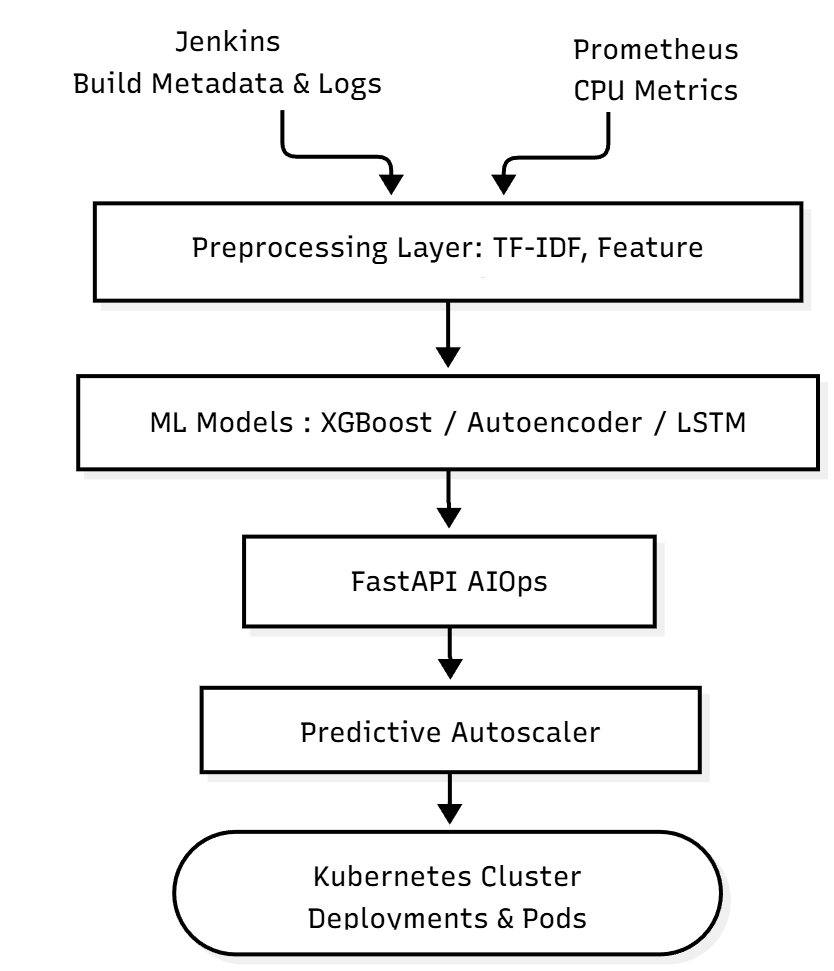
\includegraphics[width=0.70\textwidth]{overview.png}
    \caption{Overall Overview of the Proposed AIOps System}
    \label{fig:system_overview}
\end{figure}

\begin{figure}[h!]
    \centering
    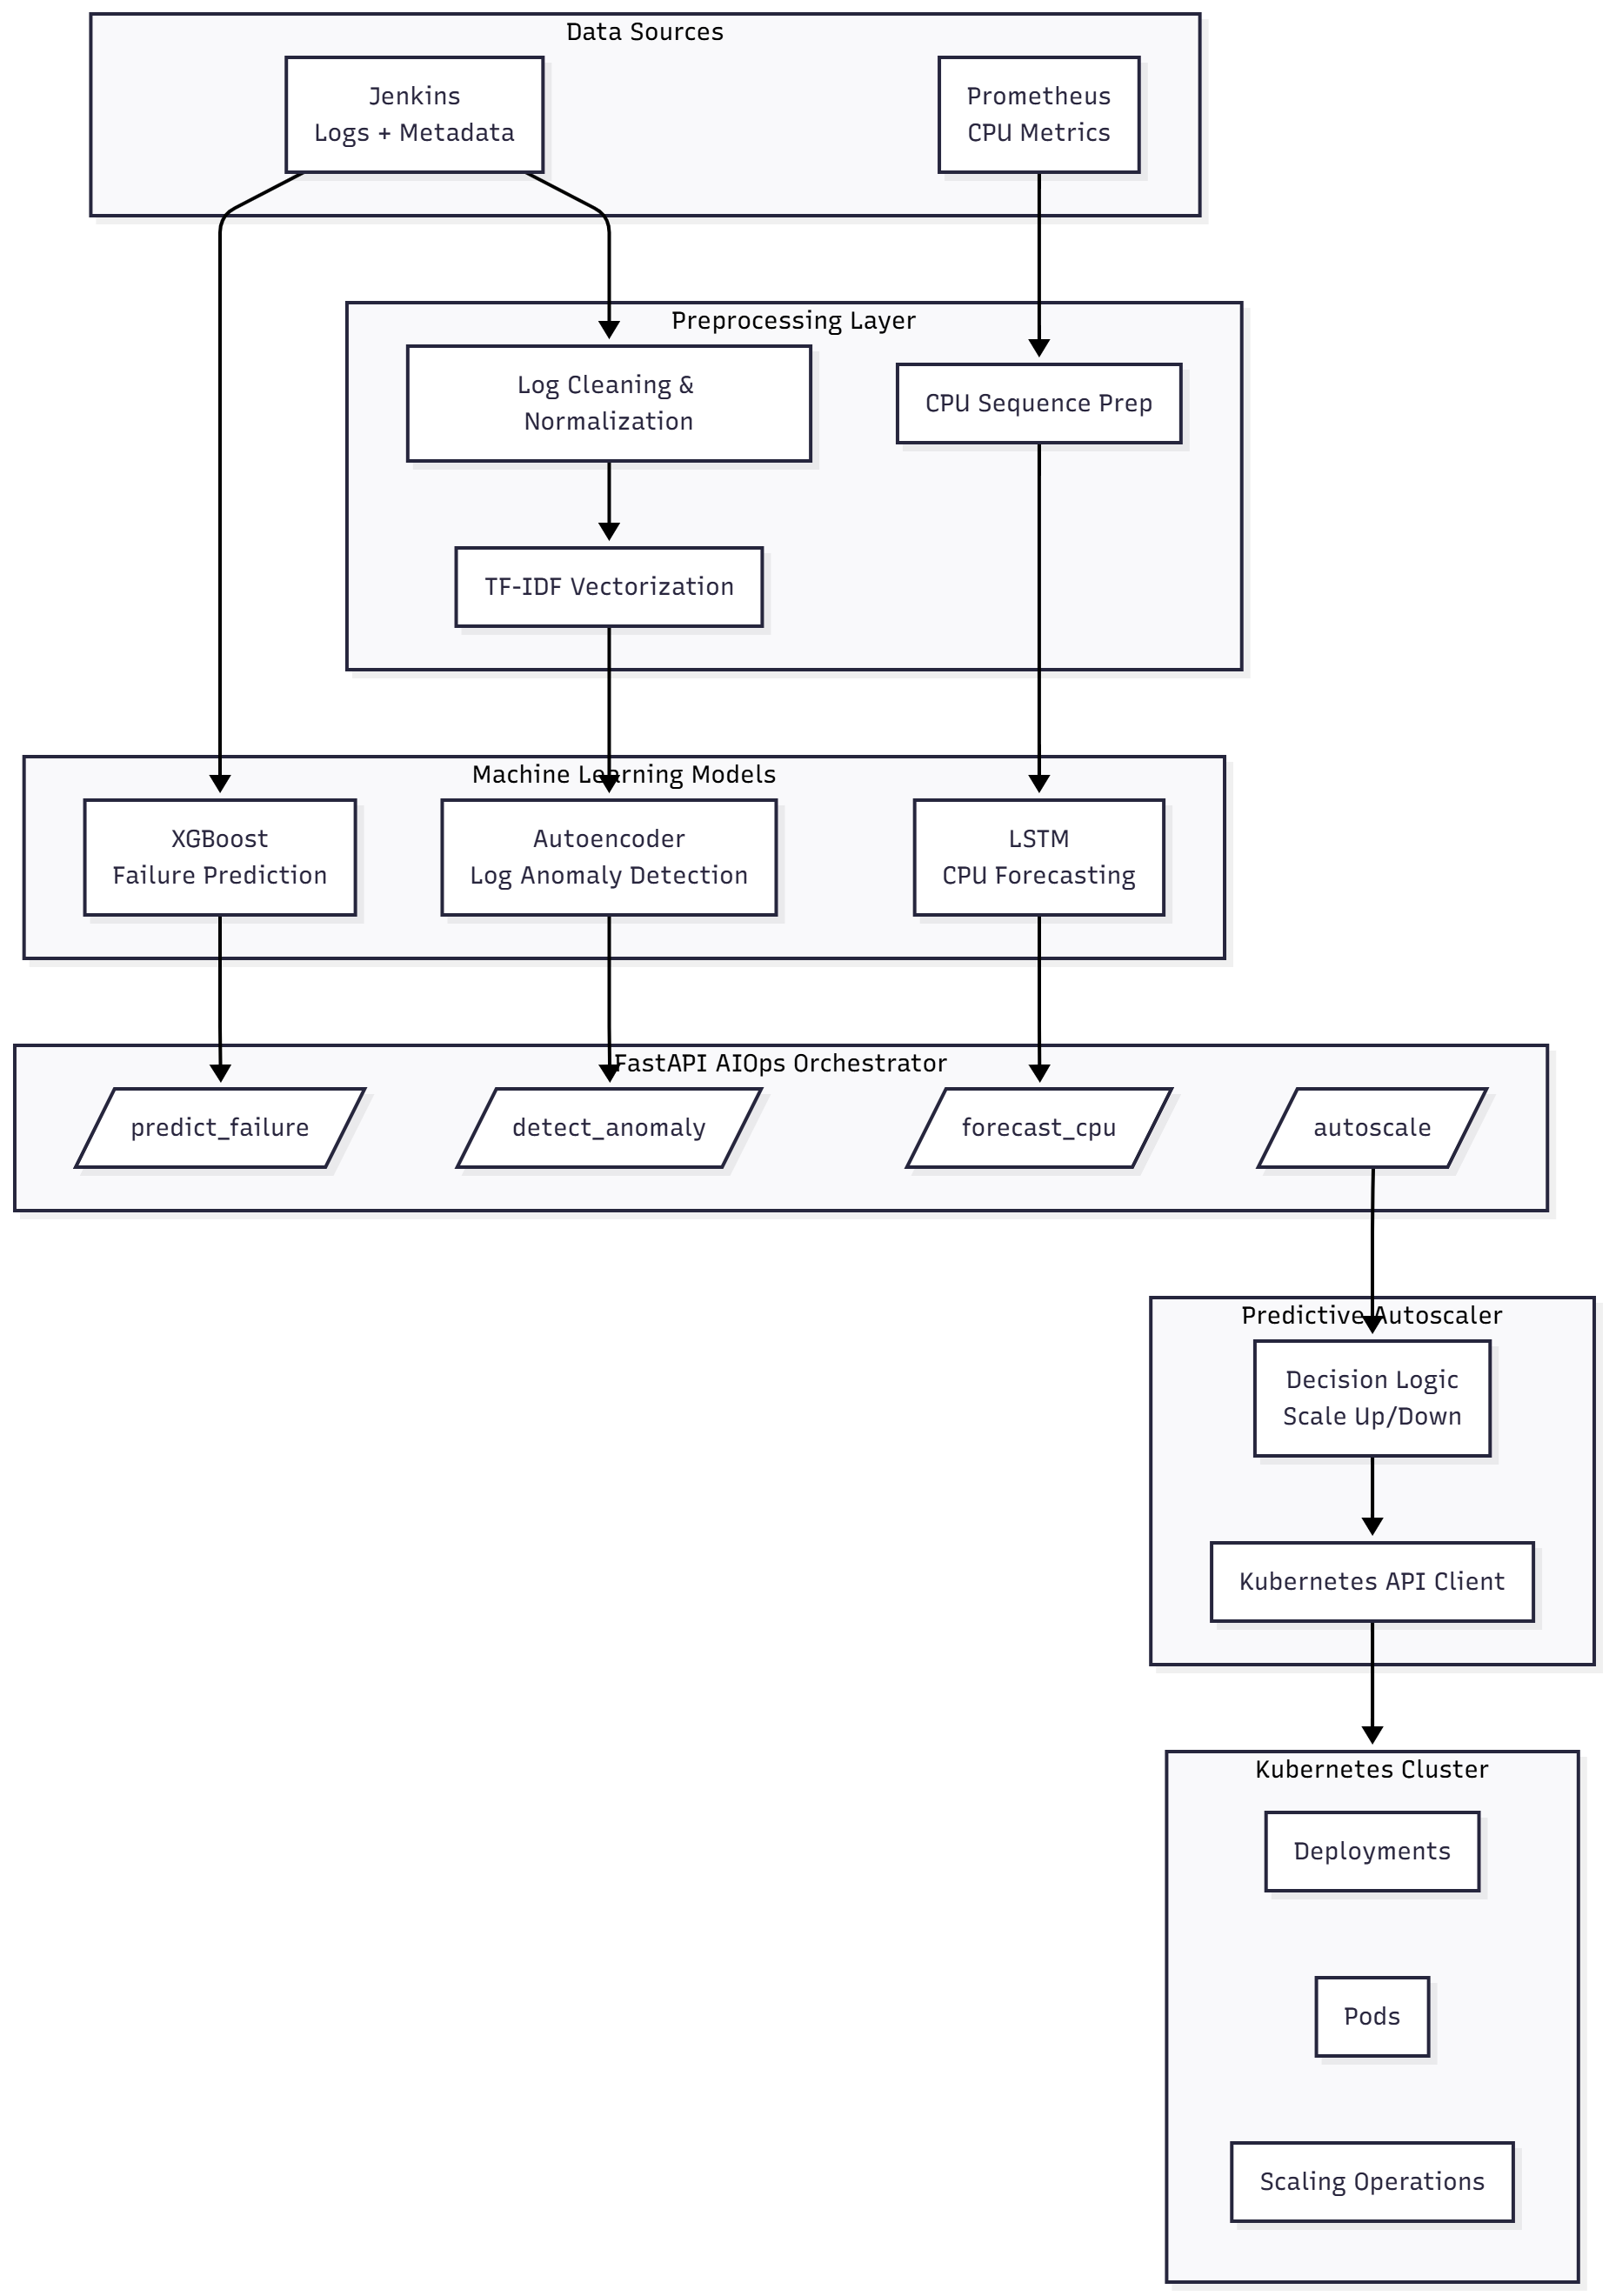
\includegraphics[width=0.9\textwidth]{architecutre.png}
    \caption{System Architecture Showing Data Flow from CI/CD to ML Pipelines and Autoscaler}
    \label{fig:system_architecture}
\end{figure}




% Chapter 5: Current Implementation Status - Page 13
\clearpage
\chapter{Current Implementation Status}

This chapter presents the work completed during Phase--II of the project. Building upon the architectural design and planning from Phase--I, this phase focused on implementing the complete data generation pipeline, training all three machine learning models, and performing a comprehensive evaluation of their performance. The implementation was carried out on a Windows environment using Python 3.10+, with TensorFlow/Keras for deep learning models and XGBoost for the classification task.

\section{Synthetic Data Generation}

Since real-world CI/CD data from Jenkins and Prometheus was limited in volume, a comprehensive synthetic data generation module was developed to produce training-ready datasets that closely mimic production CI/CD environments. The data generator (\texttt{training/generate\_synthetic\_data.py}) produces three categories of synthetic data:

\begin{itemize}
    \item \textbf{Jenkins Build Metadata:} 600 synthetic build records were generated with realistic distributions across SUCCESS ($\sim$67\%), FAILURE ($\sim$25\%), and UNSTABLE ($\sim$8\%) outcomes. Each record includes features such as duration, number of warnings, errors, test results (failed, passed, total), and log length. Feature correlations were carefully designed --- for example, failed builds tend to have longer durations, more errors, and more test failures.
    
    \item \textbf{Jenkins Console Logs:} Over 600 synthetic log files were generated using realistic templates that replicate actual Jenkins pipeline output. Logs include stages such as checkout, dependency installation, linting, testing, and build steps. Failure and success logs have distinct patterns, making them suitable for anomaly detection training with TF--IDF vectorization.
    
    \item \textbf{Prometheus CPU Time-Series:} Over 10,000 CPU usage data points were generated as a time-series with realistic patterns including diurnal cycles, random spikes, gradual trends, and noise. This dataset was used for training the LSTM forecasting model with a sliding-window approach.
\end{itemize}

\section{Data Collection Infrastructure}

In addition to synthetic data, a complete data collection infrastructure was implemented to enable future integration with live Jenkins and Prometheus instances:

\begin{itemize}
    \item \textbf{Jenkins Collector} (\texttt{collectors/jenkins\_collector.py}): A Python module that connects to Jenkins via its REST API using HTTP Basic Authentication. It retrieves build metadata (result, duration, timestamp), console logs, and test reports for specified jobs. Collected data is stored as structured CSVs and individual log files.
    
    \item \textbf{Prometheus Collector} (\texttt{collectors/prometheus\_collector.py}): A module that queries the Prometheus HTTP API to fetch time-series metrics such as CPU utilization, memory usage, and pod replica counts. It supports both instant and range queries using PromQL and exports results in structured CSV format.
    
    \item \textbf{Real-Time Collector} (\texttt{collectors/realtime\_collector.py}): A streaming collector designed for continuous, near-real-time data ingestion from both Jenkins and Prometheus sources.
\end{itemize}

\section{Model Training}

All three machine learning models were trained using the prepared datasets. Each model was implemented as a standalone training script with clear preprocessing, training, evaluation, and model serialization stages.

\subsection{XGBoost Failure Prediction Model}

The XGBoost classifier was trained on Jenkins build metadata to predict whether a CI/CD build will fail before execution. The training pipeline (\texttt{training/train\_failure\_xgboost.py}) includes:

\begin{itemize}
    \item \textbf{Input Features:} duration, warnings, errors, failures, log\_length, tests\_failed, tests\_passed, tests\_total (8 features total).
    \item \textbf{Target Variable:} Binary classification --- 1 for FAILURE, 0 for SUCCESS.
    \item \textbf{Train/Test Split:} 80\%/20\% stratified split with random seed 42.
    \item \textbf{Hyperparameters:} 100 estimators, max depth 6, learning rate 0.1, subsample 0.8, colsample\_bytree 0.8, with automatic class weight balancing using \texttt{scale\_pos\_weight}.
    \item \textbf{Output:} Trained model saved as \texttt{orchestrator/models/xgboost\_failure.bin}.
\end{itemize}

\subsection{TF--IDF + Autoencoder Log Anomaly Detection Model}

The anomaly detection model uses a two-stage pipeline: TF--IDF vectorization of Jenkins console logs followed by an Autoencoder neural network for reconstruction-based anomaly detection. The training pipeline (\texttt{training/train\_log\_anomaly.py}) includes:

\begin{itemize}
    \item \textbf{Text Vectorization:} TF--IDF vectorizer with 500 features, ngram range (1, 2), sublinear TF scaling, and English stop word removal.
    \item \textbf{Autoencoder Architecture:} Input(500) $\rightarrow$ Dense(128, ReLU) $\rightarrow$ BatchNorm $\rightarrow$ Dropout(0.3) $\rightarrow$ Dense(64, ReLU) $\rightarrow$ BatchNorm $\rightarrow$ Dropout(0.3) $\rightarrow$ Dense(32, ReLU) [bottleneck] $\rightarrow$ Dense(64, ReLU) $\rightarrow$ BatchNorm $\rightarrow$ Dropout(0.3) $\rightarrow$ Dense(128, ReLU) $\rightarrow$ BatchNorm $\rightarrow$ Dropout(0.3) $\rightarrow$ Dense(500, Sigmoid).
    \item \textbf{Training:} Trained only on normal (non-anomalous) logs using MSE loss with Adam optimizer (lr=0.0005). Early stopping with patience of 5 epochs on validation loss.
    \item \textbf{Anomaly Threshold:} Determined at the 95th percentile of reconstruction errors on normal training data.
    \item \textbf{Output:} TF--IDF vectorizer (\texttt{tfidf.pkl}), Autoencoder (\texttt{autoencoder.keras}), and threshold (\texttt{anomaly\_threshold.pkl}) saved to \texttt{orchestrator/models/}.
\end{itemize}

\subsection{LSTM CPU Forecasting Model}

The LSTM model was trained on Prometheus CPU time-series data to forecast future CPU usage. The training pipeline (\texttt{training/train\_cpu\_lstm.py}) includes:

\begin{itemize}
    \item \textbf{Data Preprocessing:} CPU values normalized to [0, 1] using MinMaxScaler. Sliding window sequences created with a lookback of 60 minutes and a forecast horizon of 10 minutes, yielding over 10,000 training sequences.
    \item \textbf{LSTM Architecture:} LSTM(128, return sequences) $\rightarrow$ Dropout(0.2) $\rightarrow$ LSTM(64) $\rightarrow$ Dropout(0.2) $\rightarrow$ Dense(32, ReLU) $\rightarrow$ Dense(1).
    \item \textbf{Training:} MSE loss with Adam optimizer (lr=0.001). Early stopping with patience of 10 epochs on validation loss, with learning rate reduction on plateau (factor 0.5, patience 5).
    \item \textbf{Output:} LSTM model (\texttt{lstm\_cpu.keras}) and scaler (\texttt{cpu\_scaler.pkl}) saved to \texttt{orchestrator/models/}.
\end{itemize}

\section{Model Evaluation Results}

A comprehensive evaluation suite (\texttt{evaluation/evaluate\_all.py}) was developed to assess all three models using standard metrics, generate publication-quality plots, and produce a consolidated metrics report.

\subsection{XGBoost Failure Prediction Results}

The XGBoost model demonstrated excellent performance on the test set:

\begin{table}[h!]
\centering
\caption{XGBoost Failure Prediction --- Test Set Performance}
\label{table:xgboost_results}
\begin{tabular}{|l|c|}
\hline
\textbf{Metric} & \textbf{Value} \\
\hline
Accuracy & 98.33\% \\
Precision & 93.10\% \\
Recall & 100.00\% \\
F1-Score & 96.43\% \\
ROC AUC & 100.00\% \\
\hline
\end{tabular}
\end{table}

A 5-fold stratified cross-validation was also performed to verify model stability:

\begin{table}[h!]
\centering
\caption{XGBoost 5-Fold Cross-Validation Results}
\label{table:xgboost_cv}
\begin{tabular}{|l|c|}
\hline
\textbf{Metric} & \textbf{Mean $\pm$ Std} \\
\hline
Accuracy & 99.00\% $\pm$ 0.62\% \\
F1-Score & 97.83\% $\pm$ 1.37\% \\
ROC AUC & 99.90\% $\pm$ 0.12\% \\
\hline
\end{tabular}
\end{table}

The confusion matrix, ROC curve, precision-recall curve, and feature importance plot were generated for detailed analysis. The feature importance analysis revealed that \texttt{errors}, \texttt{failures}, and \texttt{tests\_failed} were the most influential predictors of build failure.

\begin{figure}[t]
    \centering
    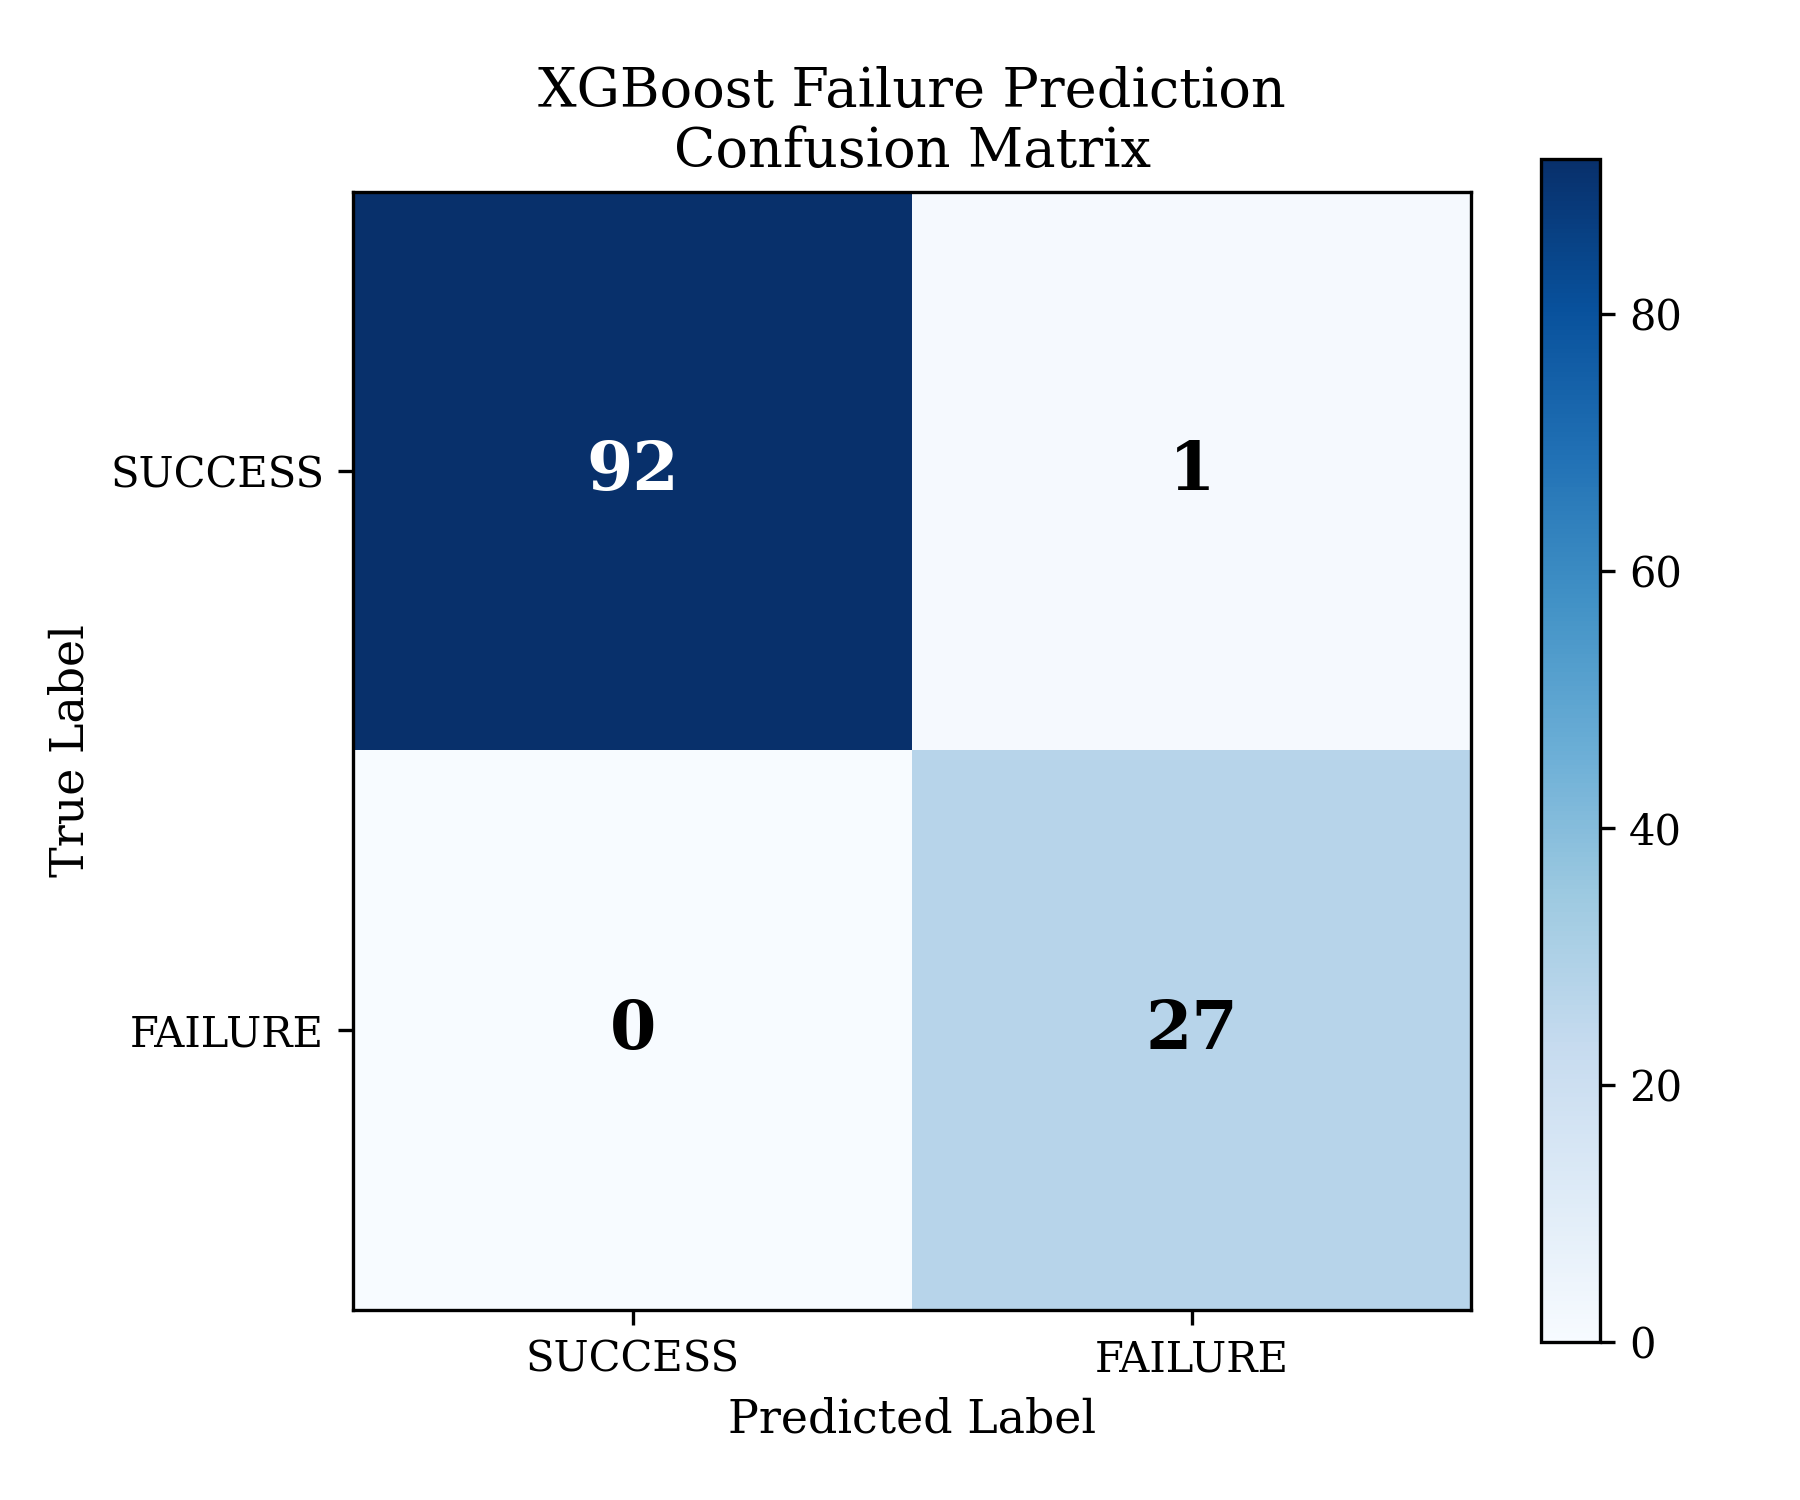
\includegraphics[width=0.55\textwidth]{xgboost_confusion_matrix.png}
    \caption{XGBoost Failure Prediction --- Confusion Matrix}
    \label{fig:xgb_cm}
\end{figure}

\begin{figure}[t]
    \centering
    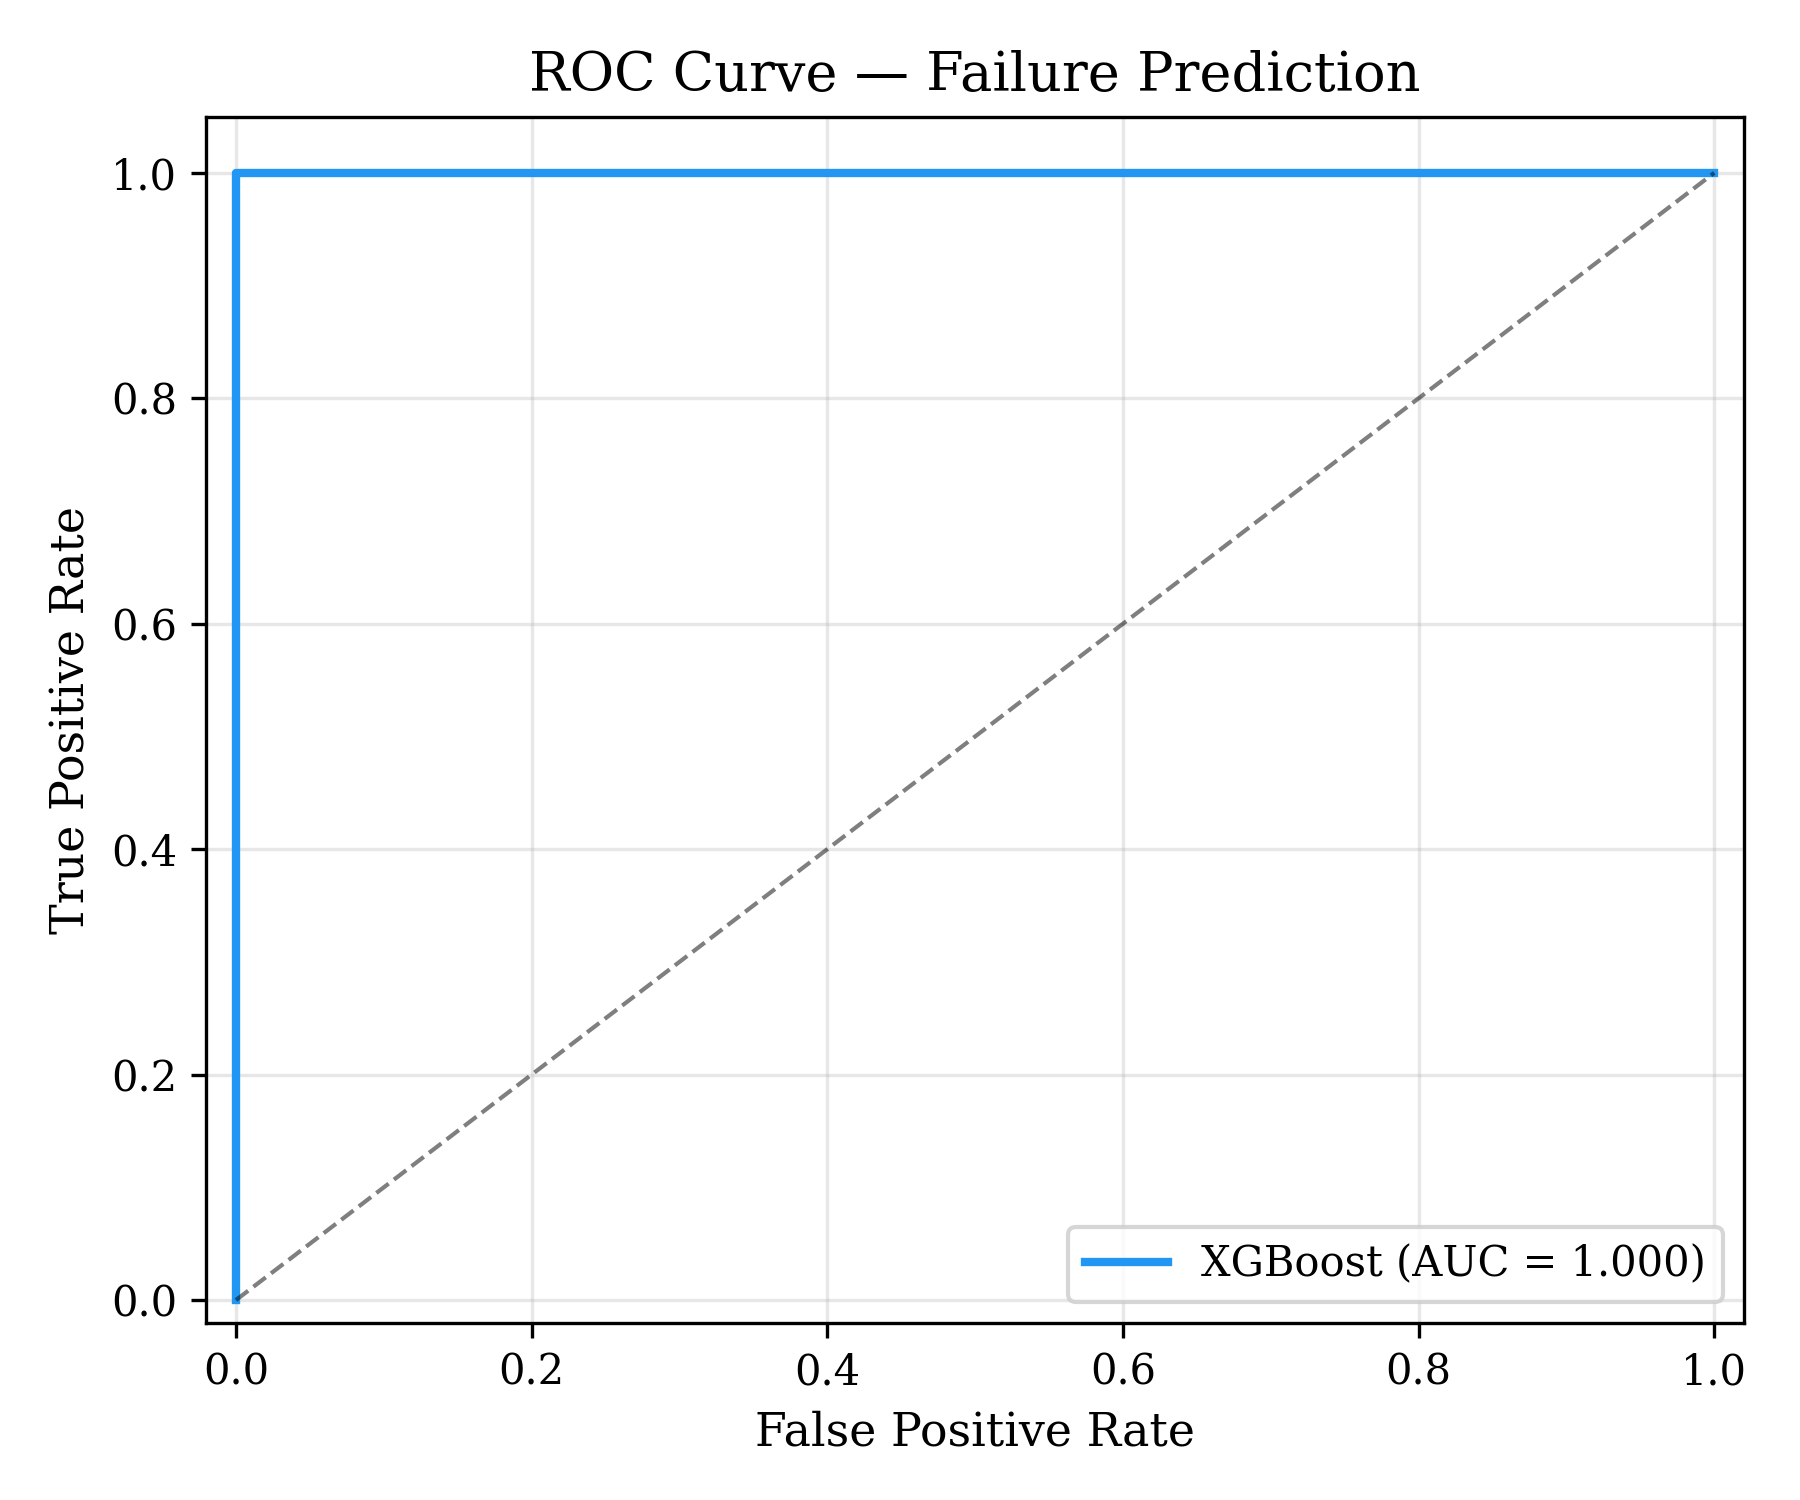
\includegraphics[width=0.55\textwidth]{xgboost_roc_curve.png}
    \caption{XGBoost Failure Prediction --- ROC Curve (AUC = 1.000)}
    \label{fig:xgb_roc}
\end{figure}

\begin{figure}[t]
    \centering
    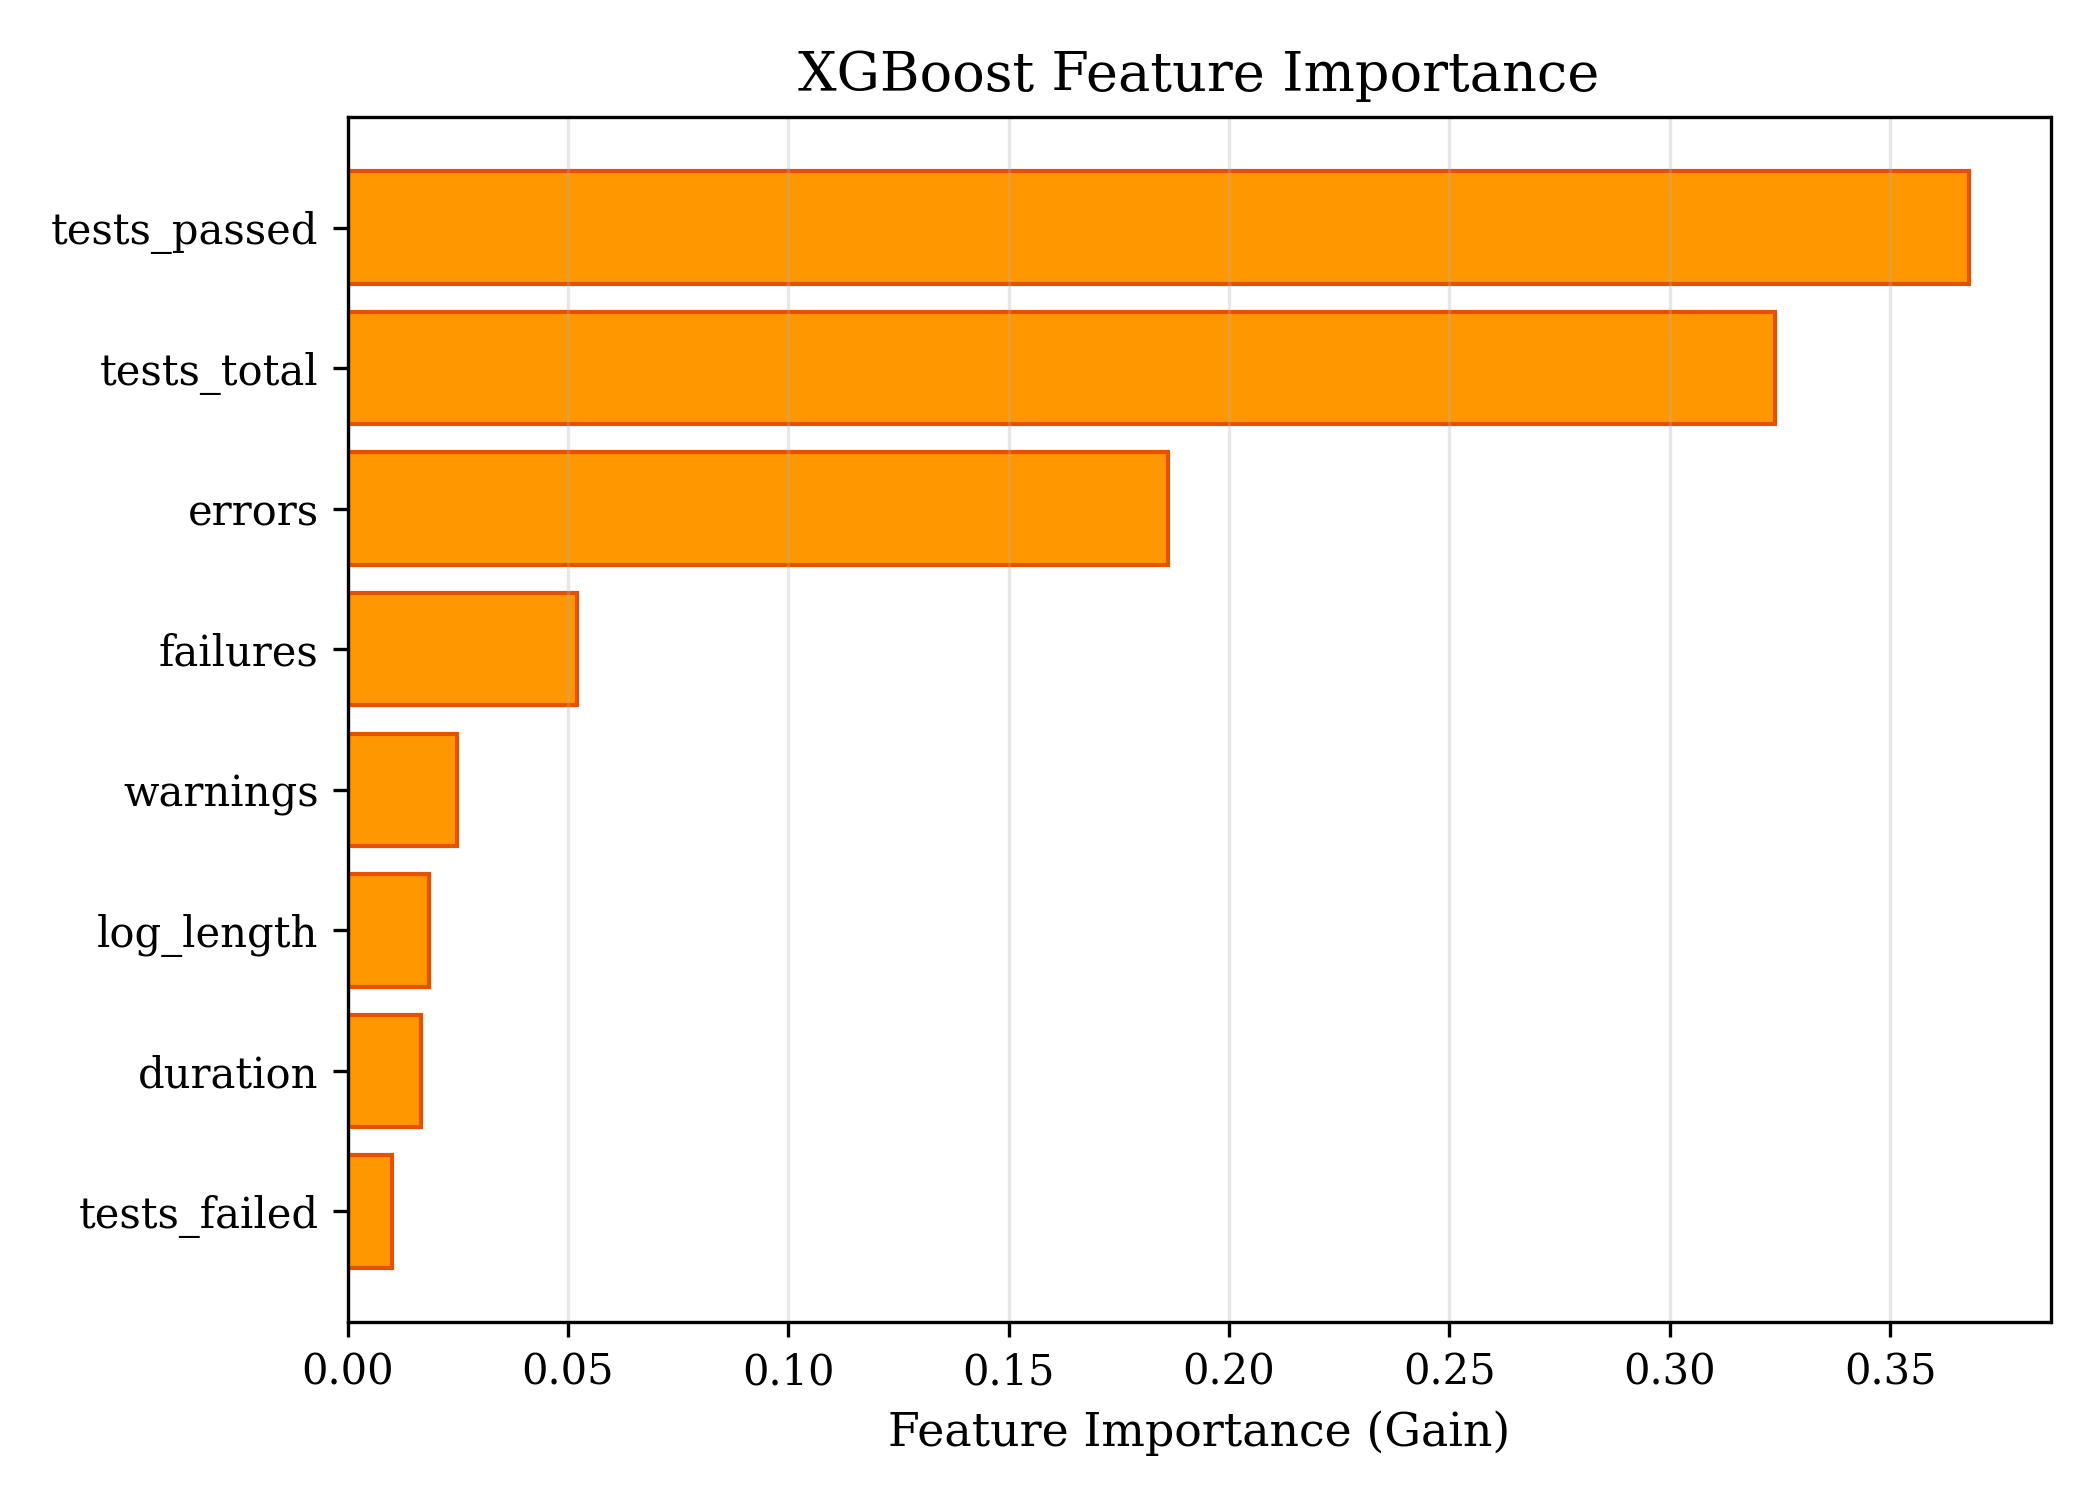
\includegraphics[width=0.60\textwidth]{xgboost_feature_importance.png}
    \caption{XGBoost Feature Importance Analysis}
    \label{fig:xgb_fi}
\end{figure}

\clearpage
\subsection{TF--IDF + Autoencoder Anomaly Detection Results}

The anomaly detection model was evaluated on a held-out test set of 121 log samples:

\begin{table}[h!]
\centering
\caption{Log Anomaly Detection --- Test Set Performance}
\label{table:anomaly_results}
\begin{tabular}{|l|c|}
\hline
\textbf{Metric} & \textbf{Value} \\
\hline
Accuracy & 95.87\% \\
Precision & 84.85\% \\
Recall & 100.00\% \\
F1-Score & 91.80\% \\
ROC AUC & 98.92\% \\
\hline
\end{tabular}
\end{table}

The model achieved perfect recall (100\%), meaning it detected all anomalous logs in the test set. The reconstruction error distribution plot shows clear separation between normal and anomalous logs, validating the effectiveness of the learned threshold.

\begin{figure}[t]
    \centering
    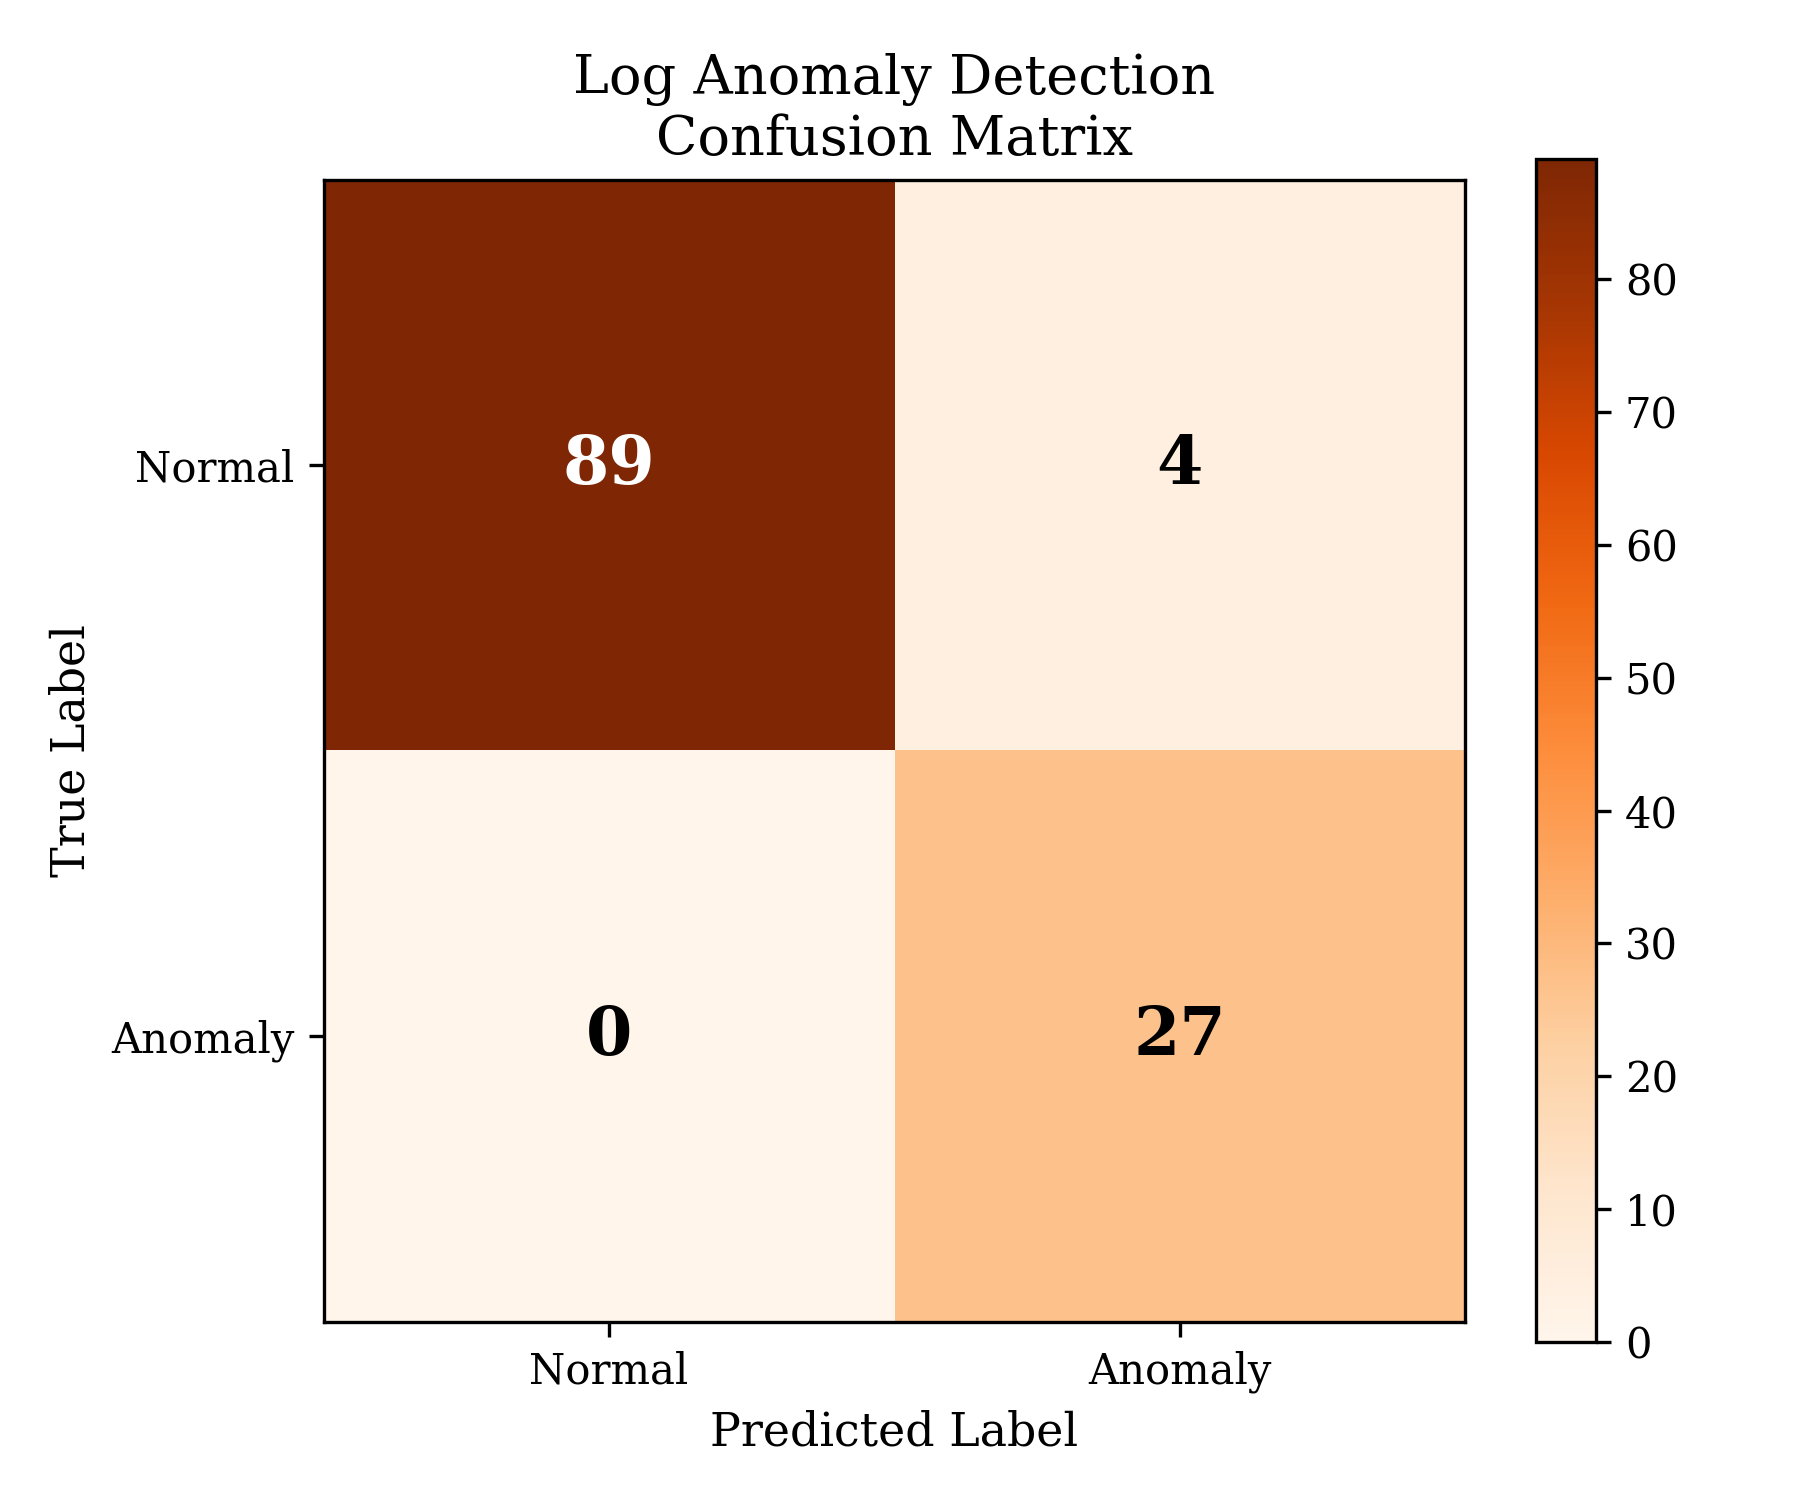
\includegraphics[width=0.55\textwidth]{anomaly_confusion_matrix.png}
    \caption{Log Anomaly Detection --- Confusion Matrix}
    \label{fig:anomaly_cm}
\end{figure}

\begin{figure}[t]
    \centering
    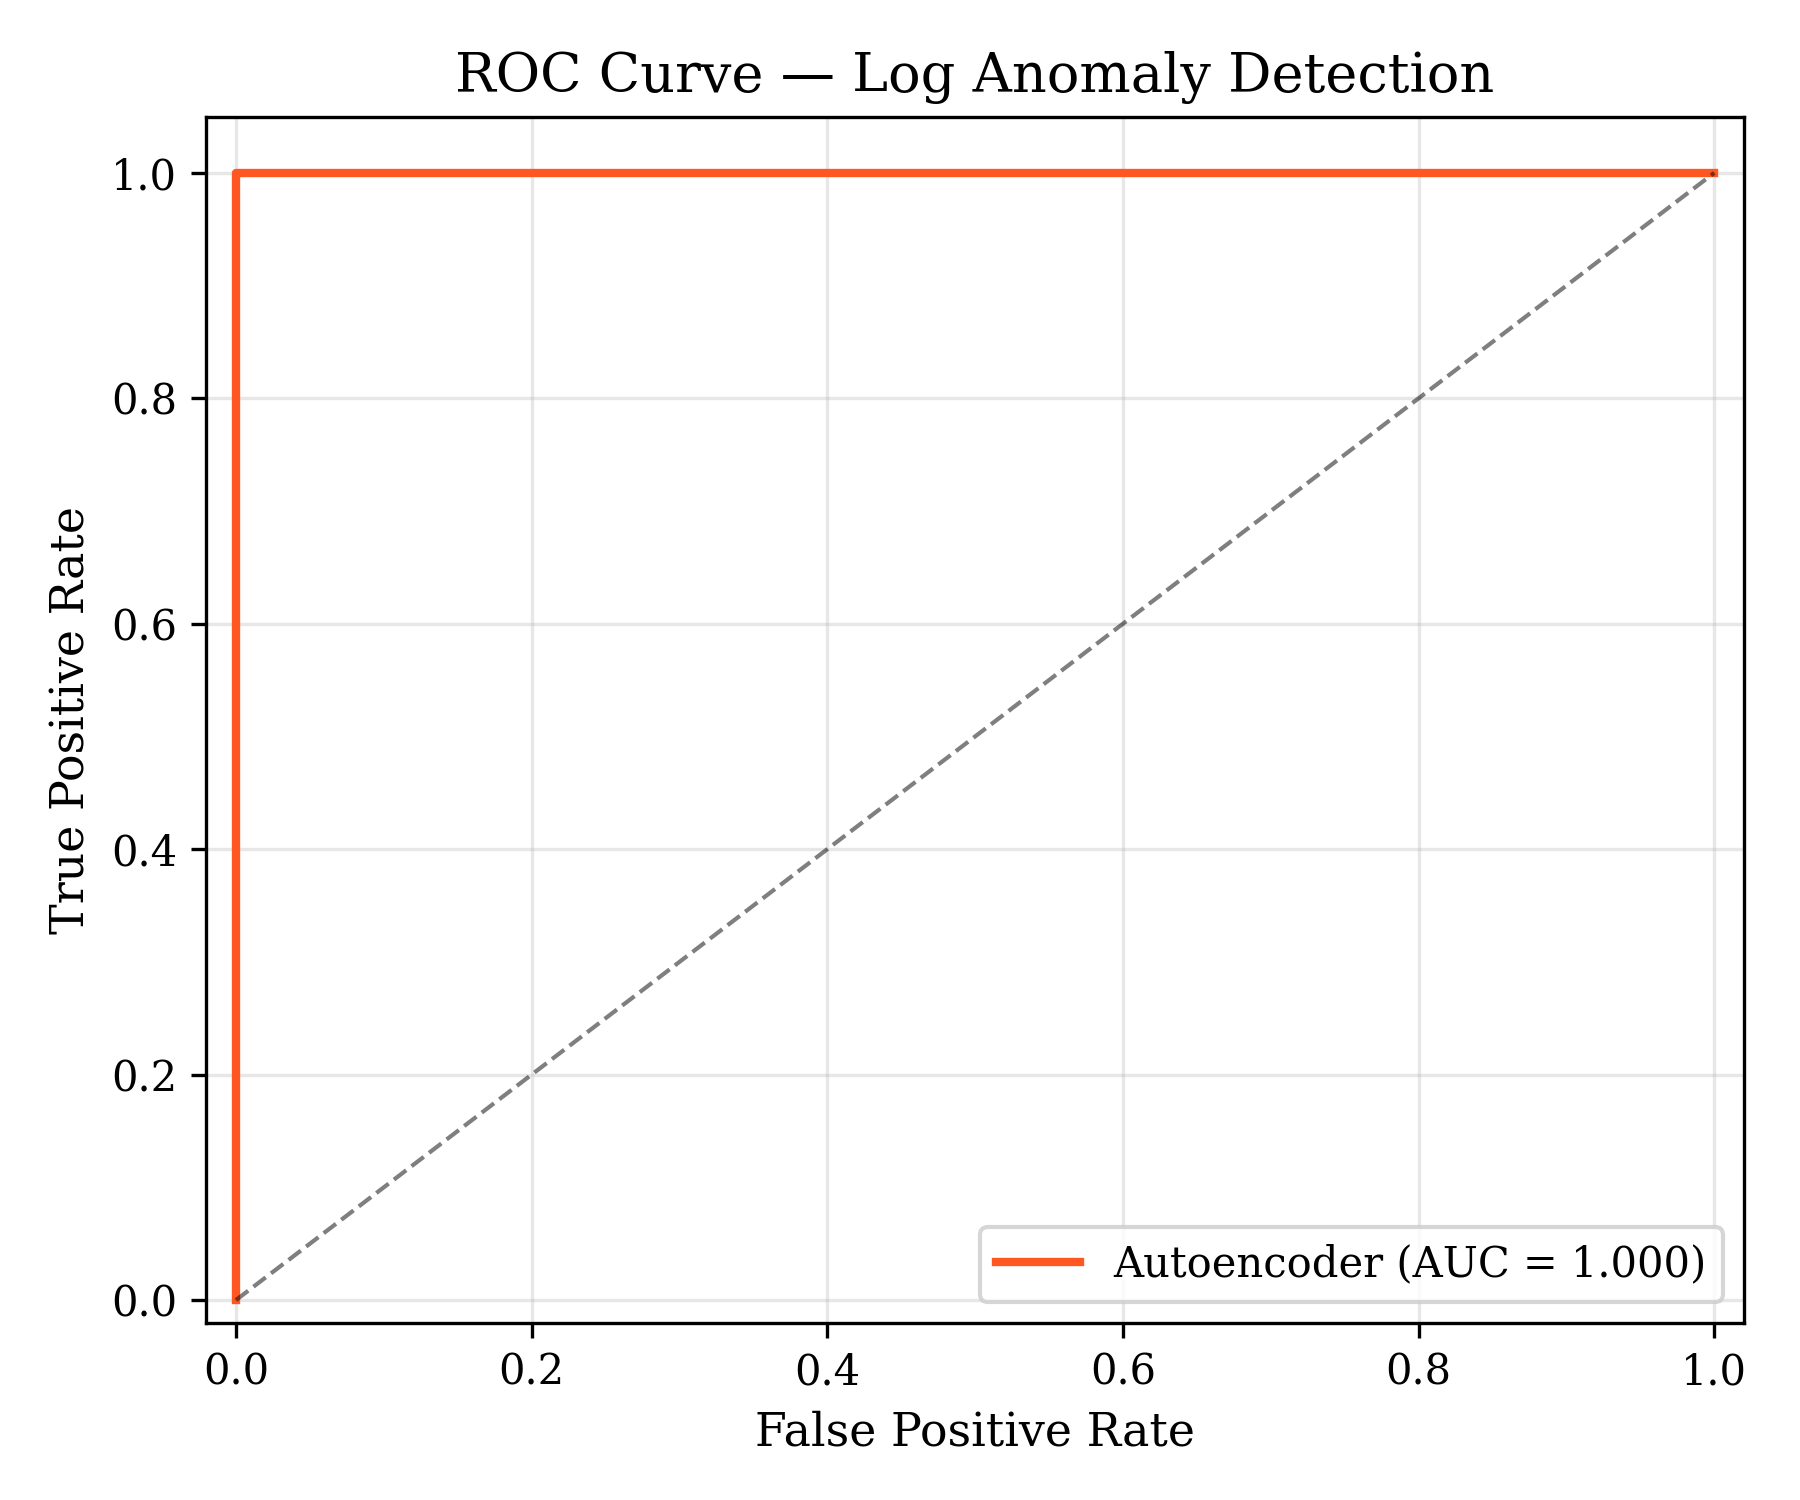
\includegraphics[width=0.55\textwidth]{anomaly_roc_curve.png}
    \caption{Log Anomaly Detection --- ROC Curve (AUC = 0.989)}
    \label{fig:anomaly_roc}
\end{figure}

\begin{figure}[t]
    \centering
    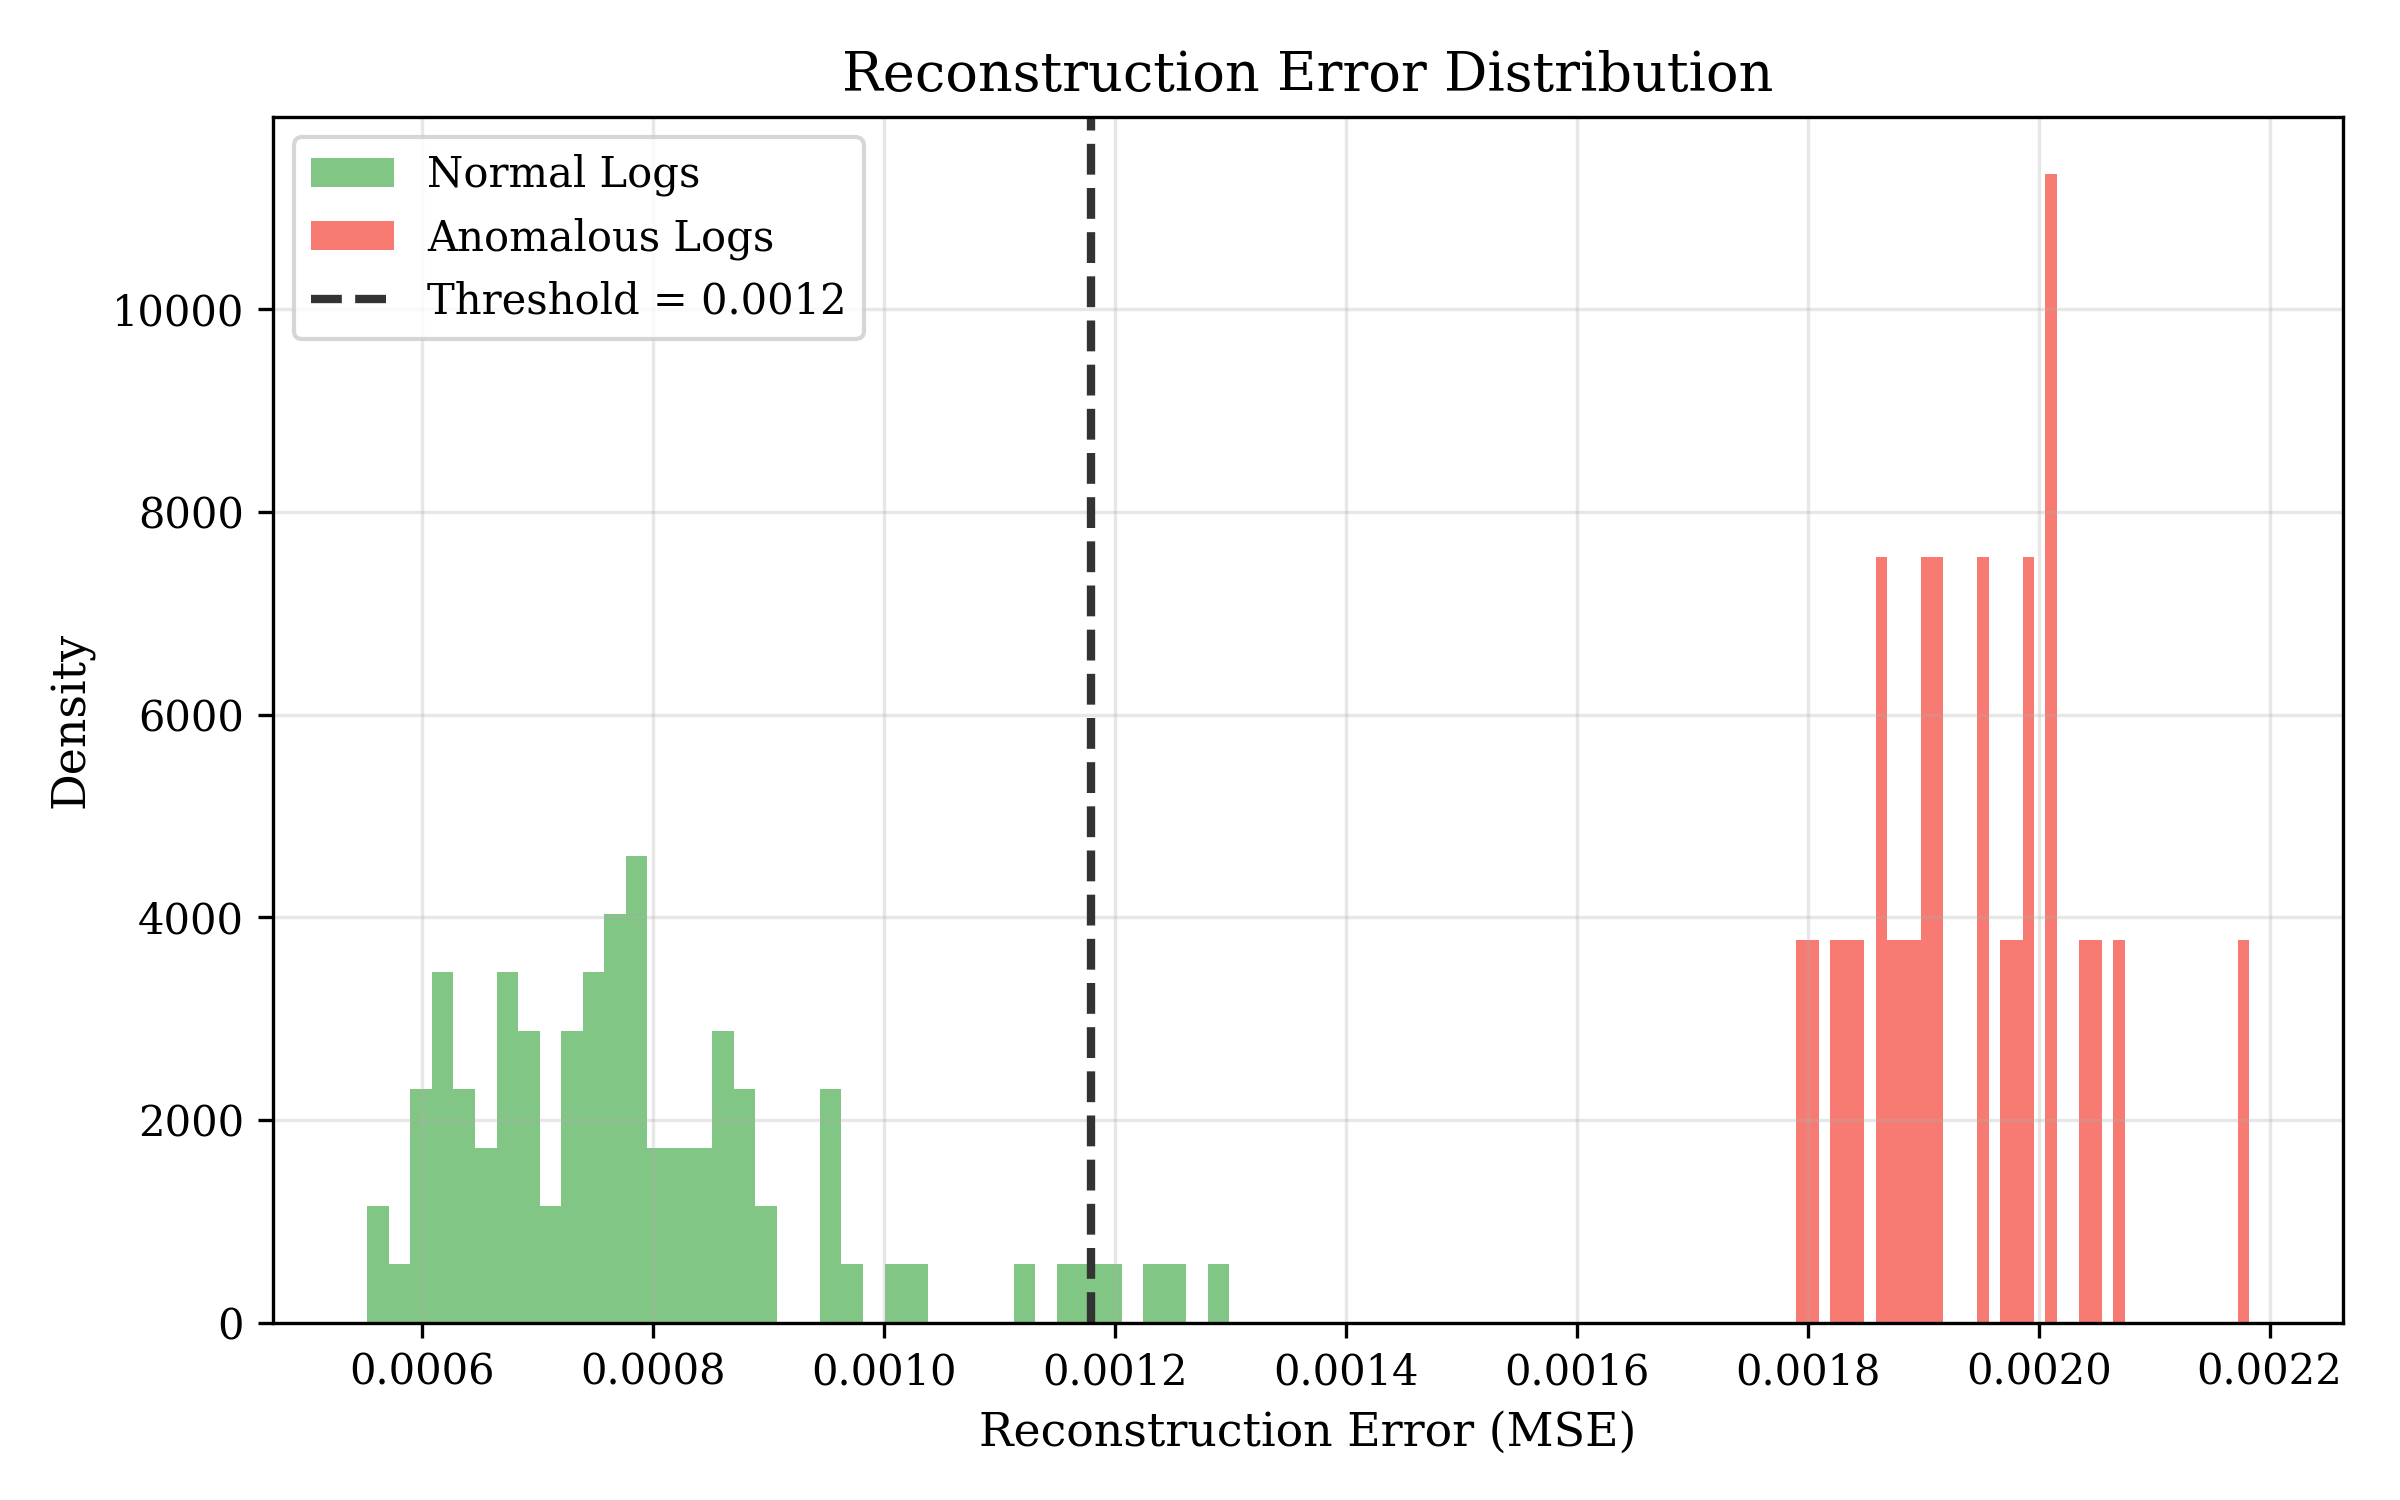
\includegraphics[width=0.65\textwidth]{anomaly_error_distribution.png}
    \caption{Reconstruction Error Distribution --- Normal vs Anomalous Logs}
    \label{fig:anomaly_dist}
\end{figure}

\clearpage
\subsection{LSTM CPU Forecasting Results}

The LSTM model was evaluated on the test portion of the CPU time-series:

\begin{table}[h!]
\centering
\caption{LSTM CPU Forecasting --- Test Set Performance}
\label{table:lstm_results}
\begin{tabular}{|l|c|}
\hline
\textbf{Metric} & \textbf{Value} \\
\hline
MSE & 0.0050 \\
MAE & 0.0436 \\
RMSE & 0.0710 \\
MAPE & 9.56\% \\
R\textsuperscript{2} & 0.435 \\
\hline
\end{tabular}
\end{table}

The model demonstrates strong short-term forecasting capability. The actual vs predicted plot and residual analysis confirm that predictions closely track real CPU trends, with residuals approximately normally distributed around zero.

\begin{figure}[t]
    \centering
    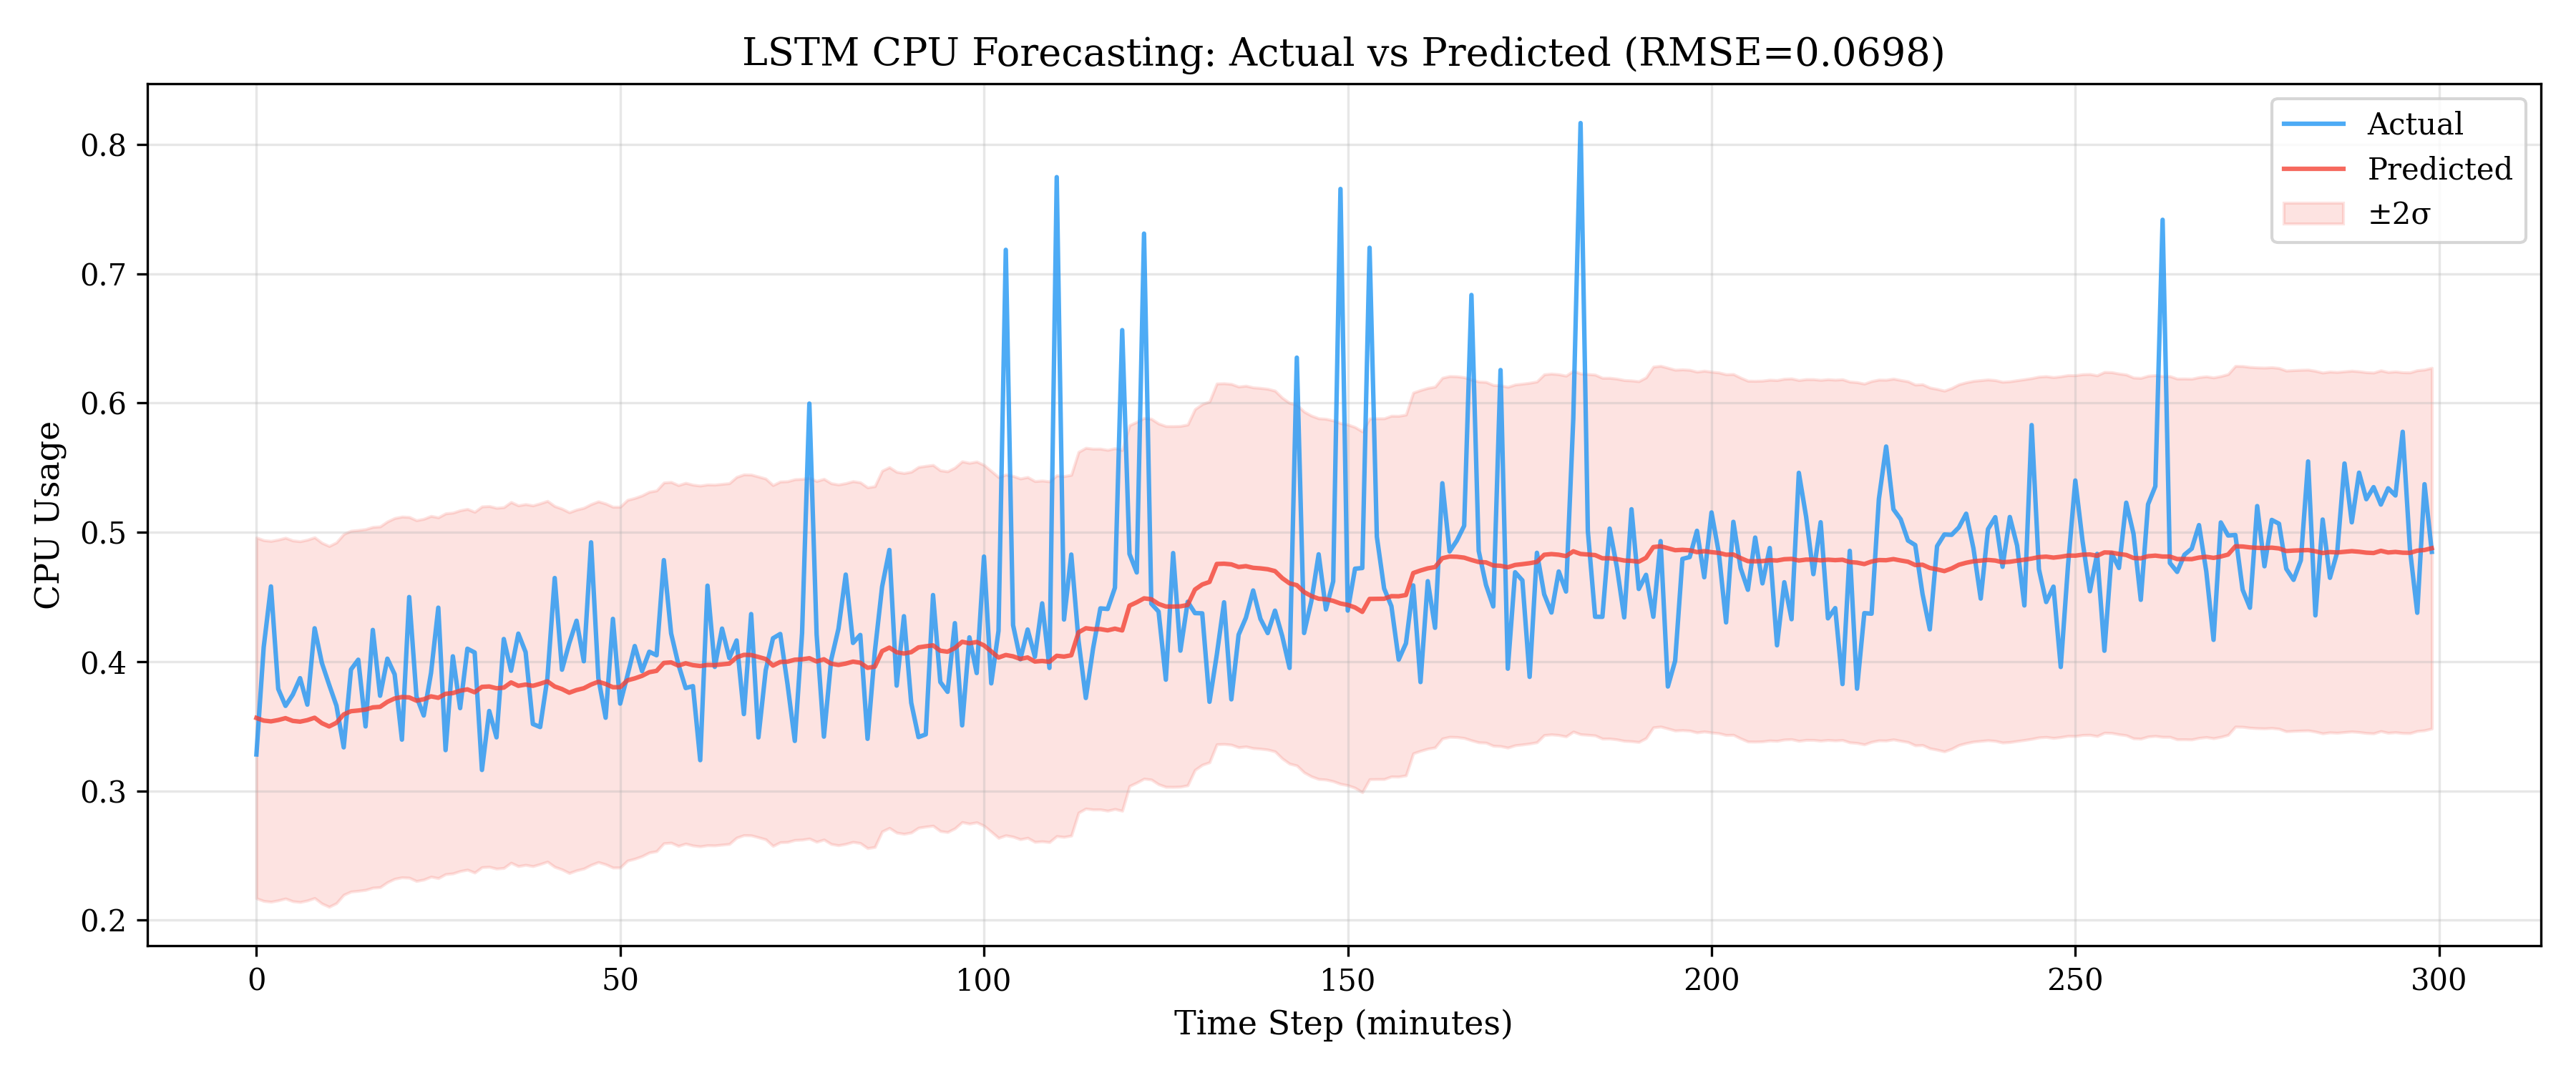
\includegraphics[width=0.75\textwidth]{lstm_actual_vs_predicted.png}
    \caption{LSTM CPU Forecasting --- Actual vs Predicted Values}
    \label{fig:lstm_pred}
\end{figure}

\begin{figure}[t]
    \centering
    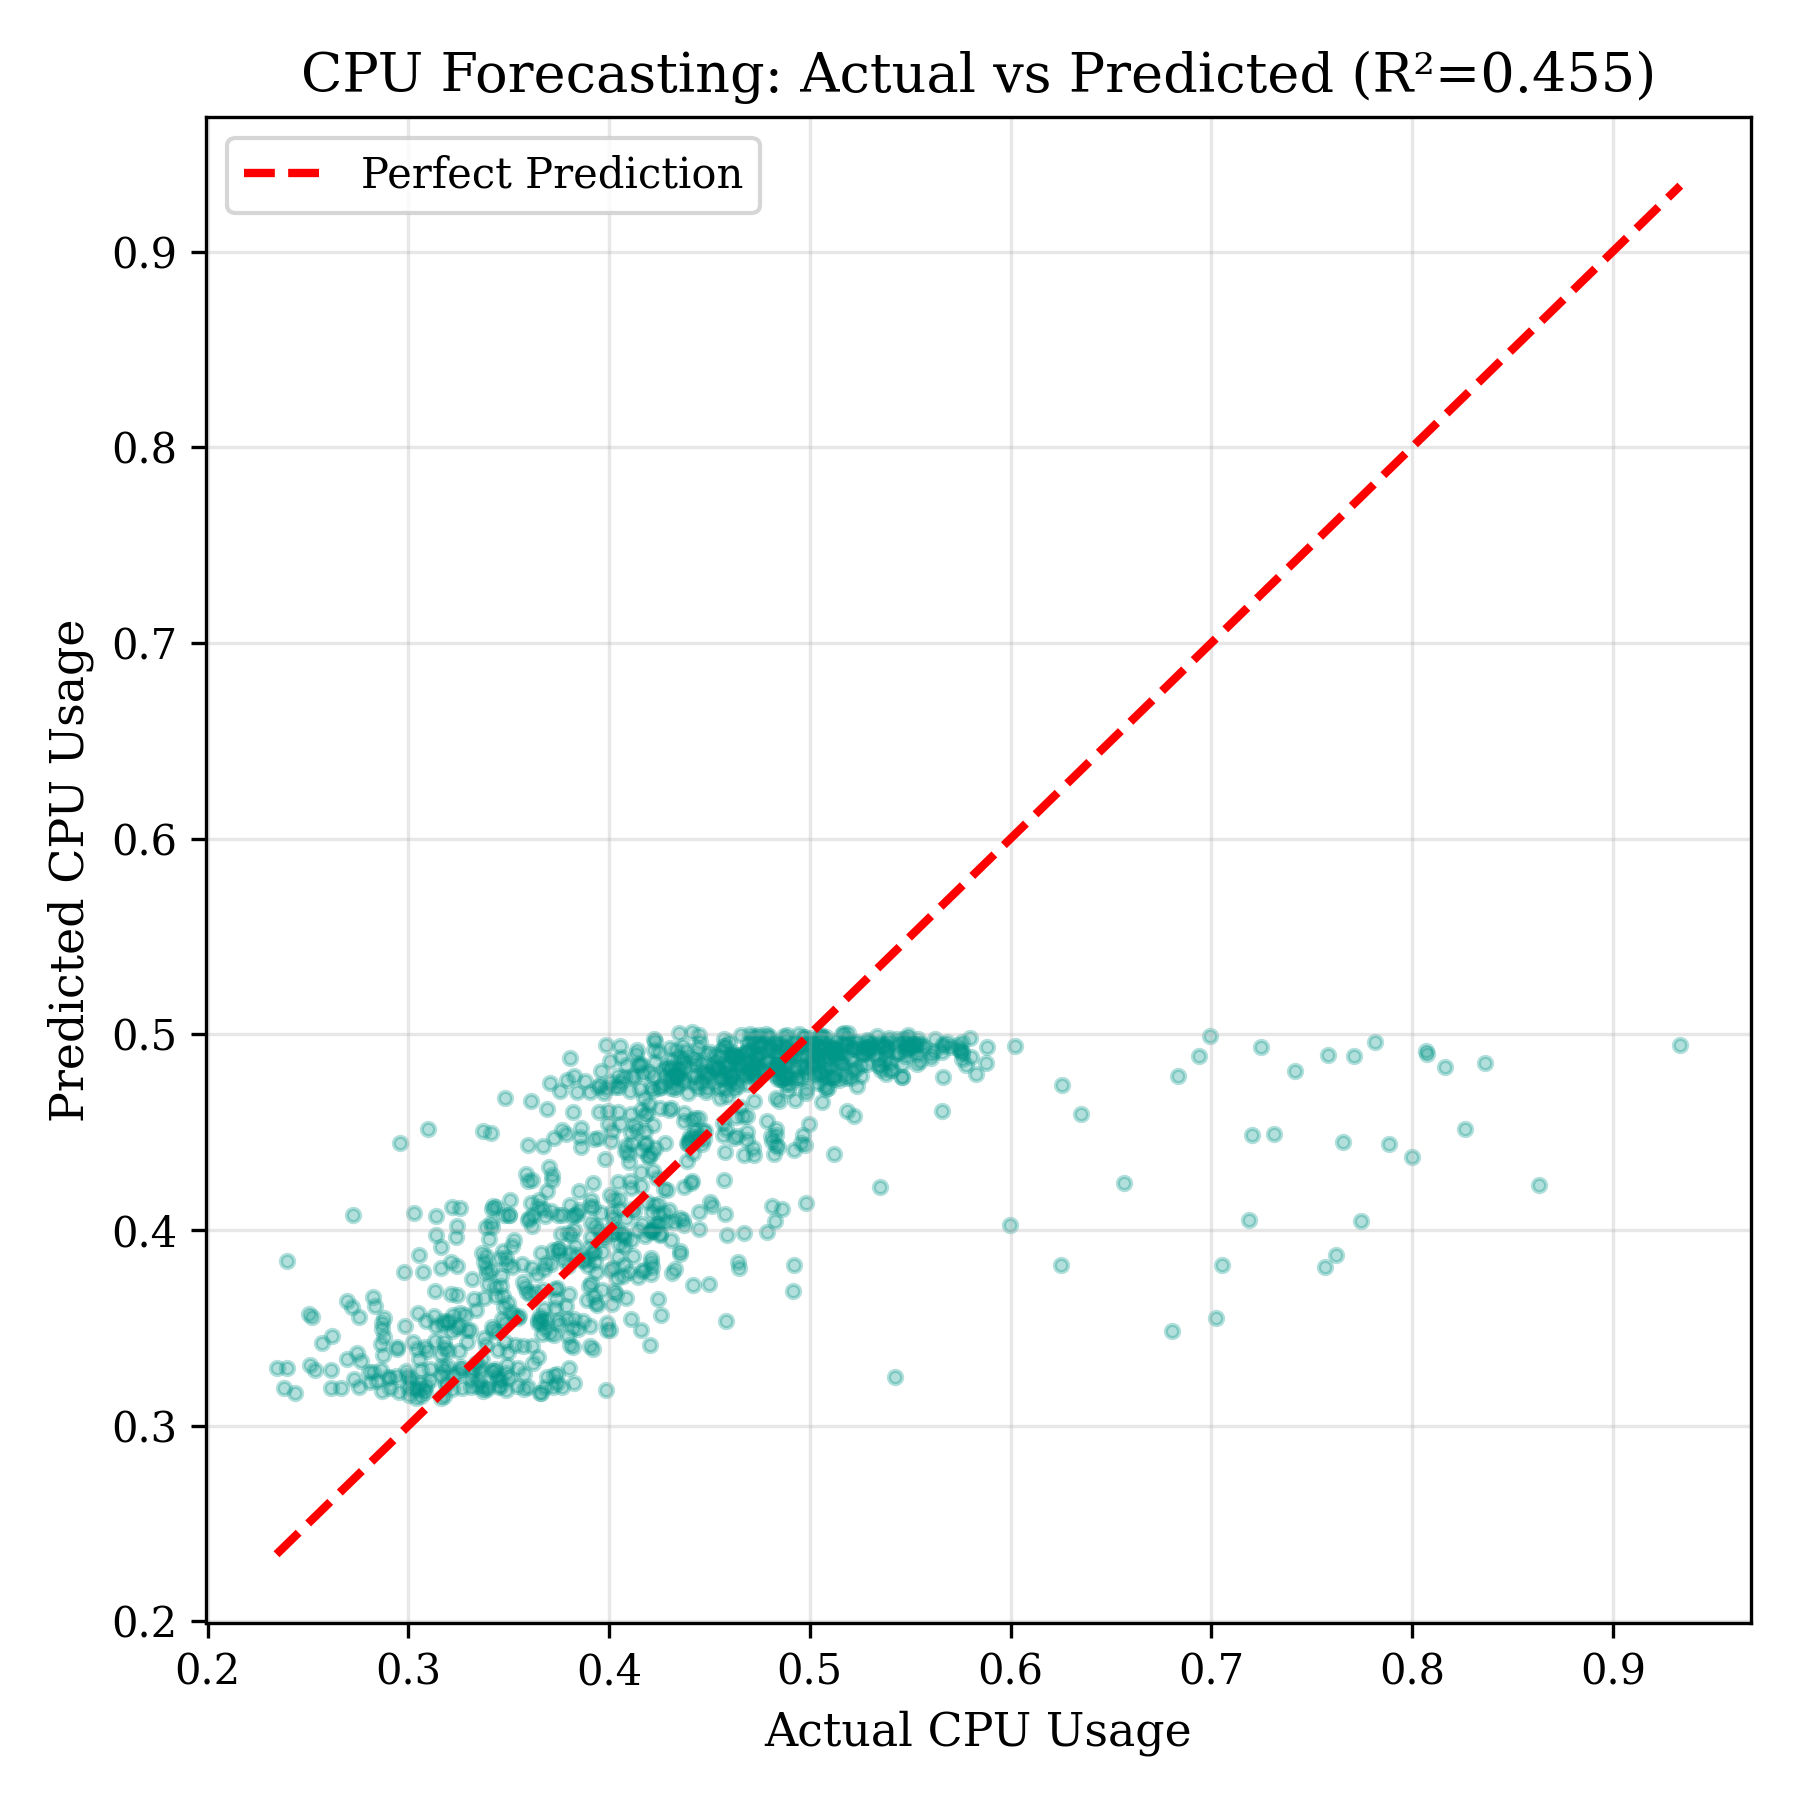
\includegraphics[width=0.50\textwidth]{lstm_scatter.png}
    \caption{LSTM CPU Forecasting --- Actual vs Predicted Scatter Plot (R\textsuperscript{2} = 0.435)}
    \label{fig:lstm_scatter}
\end{figure}

\clearpage
\subsection{Combined Model Performance Summary}

Table~\ref{table:combined_summary} presents a consolidated view of all three model performances.

\begin{table}[h!]
\centering
\caption{AIOps System --- Combined Model Performance Summary}
\label{table:combined_summary}
\begin{tabular}{|p{3.5cm}|p{3.5cm}|p{3cm}|p{3cm}|}
\hline
\textbf{Module} & \textbf{Algorithm} & \textbf{Key Metric} & \textbf{ROC AUC / R\textsuperscript{2}} \\
\hline
Failure Prediction & XGBoost & F1 = 0.964 & AUC = 1.000 \\
\hline
Anomaly Detection & TF--IDF + Autoencoder & F1 = 0.918 & AUC = 0.989 \\
\hline
CPU Forecasting & LSTM & RMSE = 0.071 & R\textsuperscript{2} = 0.435 \\
\hline
\end{tabular}
\end{table}

\begin{figure}[t]
    \centering
    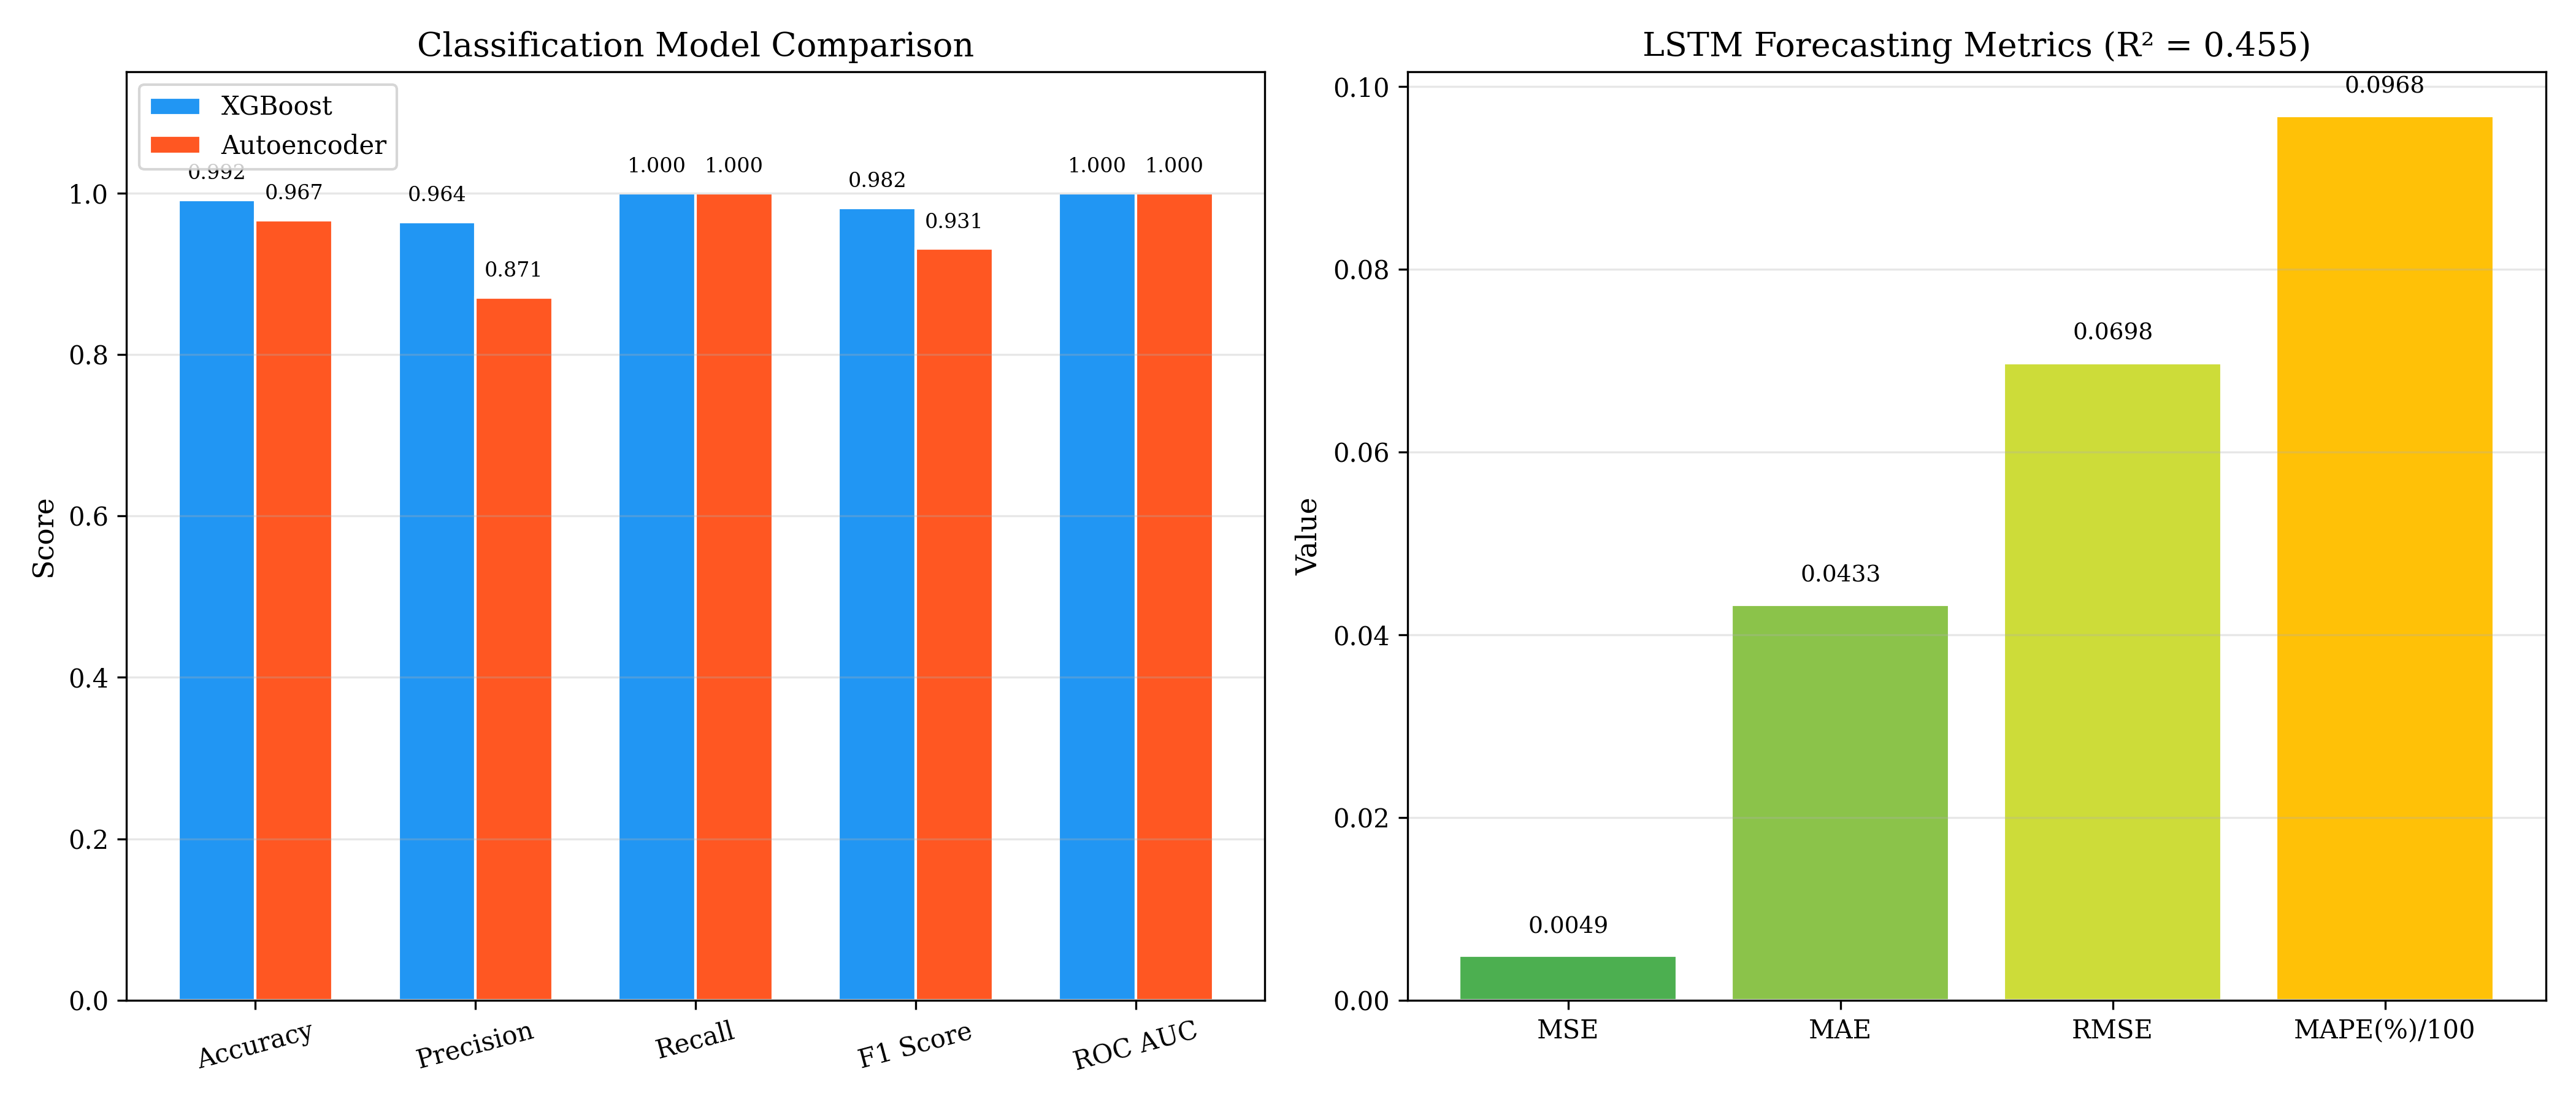
\includegraphics[width=0.80\textwidth]{model_comparison_summary.png}
    \caption{Model Comparison --- Classification Metrics and Forecasting Metrics}
    \label{fig:model_comparison}
\end{figure}

\section{Summary of Work Completed in Phase--II}

The following milestones were achieved during this phase:

\begin{itemize}
    \item Complete implementation of synthetic data generation pipeline for Jenkins builds, console logs, and CPU time-series.
    \item Development of data collection modules for Jenkins REST API and Prometheus HTTP API.
    \item Training of the XGBoost failure prediction model with 98.3\% accuracy and 96.4\% F1-score.
    \item Training of the TF--IDF + Autoencoder log anomaly detection model with 95.9\% accuracy and 91.8\% F1-score.
    \item Training of the LSTM CPU forecasting model with RMSE of 0.071 and MAPE of 9.56\%.
    \item Comprehensive evaluation suite producing 12 publication-quality plots and consolidated metrics.
    \item All trained models serialized and saved to \texttt{orchestrator/models/} for integration in the next phase.
\end{itemize}



% Chapter 6: Concrete Future Plan - Page 14
\clearpage
\chapter{Concrete Future Plan}

This chapter outlines the remaining work planned for Phase--III, the final stage of the dissertation. With all three machine learning models now trained and evaluated, the next phase focuses on integrating these models into a unified operational system, deploying predictive autoscaling on Kubernetes, and performing end-to-end validation.

\section{Phase--III: System Integration and Deployment}

\begin{enumerate}
    \item \textbf{Integration of ML Models with FastAPI Orchestrator}  
    All three trained models (XGBoost failure predictor, TF--IDF Autoencoder anomaly detector, and LSTM CPU forecaster) will be connected to the FastAPI-based AIOps orchestrator. The orchestrator will load models at startup and expose RESTful APIs: \texttt{/predict\_failure}, \texttt{/detect\_anomaly}, \texttt{/forecast\_cpu}, and \texttt{/autoscale}. This will enable real-time inference from external systems.
    
    \item \textbf{Implementation of Predictive Autoscaler}  
    A complete decision engine will be implemented that consumes ML model outputs (failure probability, anomaly score, CPU forecast) and makes proactive scaling decisions for Kubernetes deployments. The autoscaler will enforce constraints including cooldown intervals, minimum/maximum replica limits, and rate-limiting to prevent scaling oscillations.
    
    \item \textbf{Kubernetes Deployment and Testing}  
    The orchestrator, autoscaler, and demo application will be containerized using Docker and deployed on a Minikube Kubernetes cluster. Kubernetes manifests have already been prepared. The predictive autoscaler will be compared against the default Horizontal Pod Autoscaler (HPA) to measure improvements in response time and resource efficiency.
    
    \item \textbf{End-to-End System Testing}  
    Functional, performance, and stress testing will be performed across the entire pipeline --- from data ingestion through model inference to autoscaling actions. Load generation scripts will simulate real-world CI/CD workloads and traffic patterns to validate system behavior under varying conditions.
    
    \item \textbf{Dashboard and Monitoring Setup}  
    A visualization dashboard (Grafana/Streamlit) will be created to display real-time predictions, detected anomalies, CPU forecasts, and autoscaling actions. Prometheus will be configured for continuous metric collection and alerting.
    
    \item \textbf{Model Optimization and Hyperparameter Tuning}  
    Based on integration testing results, each ML model will be further optimized through hyperparameter tuning, retraining with additional data, and validation to improve accuracy, stability, and inference speed.
    
    \item \textbf{Documentation, Report Completion, and Deployment Guide}  
    All source code, system diagrams, evaluation results, integration test reports, and deployment instructions will be compiled into the final dissertation and project repository.
\end{enumerate}



\begin{thebibliography}{00}
\addcontentsline{toc}{chapter}{Bibliography}

\bibitem{pintye2024} 
I.~Pintye, B.~Goldschmidt, P.~Holicza and A.~Kertesz, 
“Enhancing Machine Learning-Based Autoscaling for Cloud Resource Orchestration,” 
\textit{Journal of Grid Computing}, vol.~22, pp.~1--18, 2024.

\bibitem{guruge2025} 
P.~B.~Guruge and Y.~H.~P.~P.~Priyadarshana, 
“Time Series Forecasting-Based Kubernetes Autoscaling Using Facebook Prophet and Long Short-Term Memory,” 
\textit{Frontiers in Computer Science}, vol.~5, 2025.

\bibitem{yahya2025} 
M.~A.~Yahya, W.~Bakhtawar and M.~Usman, 
“Deep Learning for Multivariate Time Series Anomaly Detection: A Survey of Reconstruction-Based Methods,” 
\textit{Artificial Intelligence Review}, 2025.

\bibitem{hrusto2023} 
A.~Hrusto, 
“Towards Optimization of Anomaly Detection in DevOps,” 
\textit{Information and Software Technology}, vol.~158, 2023.

\bibitem{das2025} 
S.~Das and P.~Raj, 
“AI-Enhanced Platform Engineering: Revolutionizing CI/CD Pipelines Through Intelligent Automation,” 
\textit{International Journal of Computer Engineering Science and Technology}, vol.~3, pp.~1--12, 2025.

\bibitem{abdelhamid2025} 
Y.~M.~Abdelhamid, W.~A.~Aziz and J.~N.~Soliman, 
“Kubernetes Autoscaling with Machine Learning Based on Traffic Load Prediction,” 
ResearchGate Preprint, May 2025.

\bibitem{mathew2025} 
R.~Mathew and S.~Baswareddy, 
“Predictive Failure Analysis in Continuous Integration Pipelines Using Ensemble Trees,” 
\textit{International Journal of Advanced Computer Science}, vol.~14, pp.~221--230, 2025.

\bibitem{guo2021} 
H.~Guo, J.~Zhou, P.~Luo and X.~Chen, 
“LogBERT: Transformer-Based Log Anomaly Detection for CI/CD Systems,” 
in \textit{Proc. 35th Conference on Software Engineering}, 2021.

\bibitem{sharma2025} 
P.~Sharma and R.~Kumar, 
“Auto-Scaling Techniques for Container Workloads in Kubernetes Clusters:A Review,” 
\textit{Journal of Cloud Computing}, vol.~12, pp.~1--15, 2025.

\bibitem{houerbi2024} 
S.~Houerbi, J.~da~Silva~Santos and A.~Zaidman, 
“Empirical Analysis on CI/CD Pipeline Evolution: Failures and Bottlenecks,” 
\textit{Journal of Software Maintenance and Evolution}, vol.~36, pp.~e2720, 2024.

\bibitem{kubernetesdocs} 
Kubernetes Documentation -  Autoscaling Concepts. 
[Online]. Available: \url{https://kubernetes.io/docs/tasks/run-application/horizontal-pod-autoscale/}

\bibitem{prometheusdocs} 
Prometheus Documentation - Querying and Metrics. 
[Online]. Available: \url{https://prometheus.io/docs/}

\bibitem{jenkinsdocs} 
Jenkins Documentation - Pipeline and REST API. 
[Online]. Available: \url{https://www.jenkins.io/doc/}

\end{thebibliography}



\end{document}